% ===========================================================================
% Architetture Dati - Elaborato d'esame
% Compilazione: latexmk -pdf report.tex   (richiede biber per la bibliografia)
% ===========================================================================
\documentclass[11pt, a4paper, oneside, numbers=noenddot]{scrreprt}

% --- Dati dell'elaborato ---------------------------------------------------
\newcommand{\titoloElaborato}{Progetto Architetture Dati - Confronto scalabilità tra DBMS relazionale e non relazionale}
\newcommand{\sottotitoloElaborato}{Valutazione empirica della scalabilità in ambiente distribuito di PostgreSQL e MongoDB}
\newcommand{\autore}{Fabio Compagnoni}
\newcommand{\matricola}{944954}
\newcommand{\ateneo}{Universit\`a degli Studi di Milano Bicocca}
\newcommand{\dipartimento}{Dipartimento di Informatica, Sistemistica e Comunicazione}
\newcommand{\corso}{Corso di Laurea Magistrale in Informatica}
\newcommand{\corsoEsame}{Architetture Dati}
\newcommand{\docente}{Prof.\ Andrea Maurino}
\newcommand{\annoacc}{2025/2026}
% --------------------------------------------------------------------------

% ---------------------------------------------------------------------------
% Preambolo: pacchetti e impostazioni tipografiche
% ---------------------------------------------------------------------------

% Lingua e codifica
\usepackage[T1]{fontenc}
\usepackage[utf8]{inputenc}
\usepackage[italian]{babel}
\usepackage{lmodern}
\usepackage{microtype}
\usepackage{indentfirst}

% Impaginazione
\usepackage[a4paper, top=3cm, bottom=3cm, left=3cm, right=2.7cm]{geometry}
\usepackage[headsepline]{scrlayer-scrpage}
\pagestyle{scrheadings}
\setlength{\emergencystretch}{2em}

% Matematica e simboli
\usepackage{amsmath}
\usepackage{amssymb}

% Figure e tabelle
\usepackage{graphicx}
\graphicspath{{figure/}}
\usepackage{pdflscape}
\usepackage{booktabs}
\usepackage{tabularx}
\usepackage{array}
\usepackage{multirow}
\usepackage{longtable}
\usepackage{caption}
\usepackage{subcaption}
\usepackage{float}
\captionsetup{font=small, labelfont=bf}
% Piazzamento float: riempire di più le pagine ed evitare pagine mezze vuote
\renewcommand{\topfraction}{0.9}
\renewcommand{\bottomfraction}{0.85}
\renewcommand{\textfraction}{0.07}
\renewcommand{\floatpagefraction}{0.75}
\setcounter{topnumber}{3}
\setcounter{totalnumber}{5}

% Numeri, unità di misura, grafici da CSV
\usepackage{siunitx}
\sisetup{output-decimal-marker={,}, group-separator={.}, per-mode=symbol}
\usepackage{pgfplots}
\usepackage{pgfplotstable}
\pgfplotsset{compat=1.18}
\usetikzlibrary{arrows.meta, positioning}

% Codice sorgente (SQL, mongosh/JS, shell)
\usepackage{listings}
\usepackage{xcolor}
\definecolor{codebg}{gray}{0.97}
\definecolor{codekw}{rgb}{0.10,0.10,0.55}
\definecolor{codecm}{rgb}{0.35,0.45,0.35}
\definecolor{codest}{rgb}{0.55,0.25,0.10}
\lstdefinestyle{sobrio}{
  backgroundcolor=\color{codebg},
  basicstyle=\ttfamily\footnotesize,
  keywordstyle=\color{codekw}\bfseries,
  commentstyle=\color{codecm}\itshape,
  stringstyle=\color{codest},
  numberstyle=\ttfamily\scriptsize\color{gray},
  numbers=left, numbersep=8pt,
  frame=single, rulecolor=\color{gray!40},
  breaklines=true, showstringspaces=false,
  tabsize=2, columns=fullflexible,
  captionpos=b,
}
\lstset{style=sobrio}

% Elenchi
\usepackage{enumitem}
\setlist{itemsep=2pt, topsep=3pt}

% Bibliografia
\usepackage[autostyle, italian=guillemets]{csquotes}
\usepackage[backend=biber, style=numeric-comp, sorting=none, giveninits=true]{biblatex}
\addbibresource{bibliografia.bib}

% Collegamenti (caricare tardi) e riferimenti incrociati
\usepackage[hidelinks, breaklinks=true]{hyperref}
\usepackage[nameinlink, italian]{cleveref}

% Font intestazioni KOMA più sobrio
\setkomafont{disposition}{\normalfont\bfseries}
\addtokomafont{chapter}{\Large}
\renewcommand*{\chapterheadstartvskip}{\vspace*{1.2\baselineskip}}

% Segnaposto da compilare (evidenziati in rosso finché presenti)
\newcommand{\TODO}[1]{\textcolor{red}{\textbf{[#1]}}}
% Nota di lavorazione: visibile solo in modalità bozza (\notebozza attivo)
\newif\ifnotebozza\notebozzafalse
\newcommand{\nota}[1]{\ifnotebozza\marginpar{\footnotesize\color{blue!60}#1}\fi}


\hypersetup{
  pdftitle={\titoloElaborato},
  pdfauthor={Fabio Compagnoni},
  pdfsubject={Progetto Architetture Dati}
}

\begin{document}

% ---------------------------------------------------------------------------
% Frontespizio
% ---------------------------------------------------------------------------
\begin{titlepage}
\centering

{\large\scshape \ateneo \par}
\vspace{2pt}
{\normalsize \dipartimento \par}
\vspace{6pt}
{\normalsize \corso \par}

\vspace{4pt}
\rule{\textwidth}{0.4pt}

\vfill

{\normalsize Elaborato per l'esame di \par}
\vspace{4pt}
{\large\bfseries \corsoEsame \par}

\vspace{1.6cm}

{\huge\bfseries \titoloElaborato \par}
\vspace{0.6cm}
{\large\itshape \sottotitoloElaborato \par}

\vfill

\begin{minipage}[t]{0.48\textwidth}
  \raggedright
  {\small\scshape Candidato}\\[2pt]
  {\large \autore}\\[2pt]
  {\small matr.\ \matricola}
\end{minipage}\hfill
\begin{minipage}[t]{0.48\textwidth}
  \raggedleft
  {\small\scshape Docente}\\[2pt]
  {\large \docente}
\end{minipage}

\vspace{1.4cm}
\rule{\textwidth}{0.4pt}
\vspace{4pt}

{\normalsize Anno Accademico \annoacc \par}

\end{titlepage}


\pagenumbering{arabic}

% 1. Introduzione: obiettivo, i due sistemi, cosa si valuta (requisiti)
\chapter{Introduzione}
\label{ch:introduzione}

Questo elaborato valuta empiricamente se e quando un DBMS distribuito sia adatto a un carico applicativo reale di tipo HR/retributivo (ditte, dipendenti, contratti, presenze e cedolini paga in regime
\emph{multitenant}), confrontando due sistemi che rappresentano filosofie opposte di gestione dei dati:

\begin{itemize}
  \item \textbf{PostgreSQL + Citus}: un DBMS \emph{relazionale} reso realmente distribuito dall'estensione
        Citus (un coordinator e $N$ worker), con schema rigido, SQL completo, transazioni ACID e consistenza
        forte;
  \item \textbf{MongoDB}: un DBMS \emph{documentale} (sharded cluster), con schema flessibile, dati
        organizzati in documenti annidati e distribuzione automatica tramite il balancer.
\end{itemize}

I due sistemi appartengono alla stessa classe rispetto al teorema CAP (entrambi \textbf{CP}) ma hanno modelli di dati molto diversi: questo permette di capire quando ciascun modello rappresenta bene questo tipo di dati e come si comportano in ambiente distribuito.

\section{Contesto e motivazione}
\label{sec:usecase}

La scelta del dominio non è casuale: nasce da una collaborazione lavorativa con un'azienda di consulenza HR,
tra i cui servizi principali c'è la creazione e l'elaborazione dei cedolini paga. Partendo da \textbf{file XML
di paghe reali}, è sorta una domanda concreta: come modellare al meglio questi dati, sia con un database
\emph{relazionale} sia con uno \emph{documentale} (non relazionale). In un contesto realistico con
\textbf{migliaia di dipendenti e di aziende}, si tratta poi di capire quale dei due sistemi si comporti meglio
e quindi quale convenga implementare in produzione.

Prima di avviare i test sono stati studiati i fondamenti teorici dei due sistemi e lette le rispettive
documentazioni ufficiali: il modello dei dati, il linguaggio di interrogazione e il modo in cui affrontano
scalabilità e transazioni concorrenti. Solo dopo si è passati alla verifica sperimentale. L'elaborato segue
questa struttura: una parte teorica (\Cref{ch:dominio}) e una sperimentale su un cluster reale
(\Cref{ch:metodologia,ch:risultati}), in cui si confronta quanto affermato in teoria con i dati misurati. Per il vincolo GDPR i dati reali non sono utilizzabili direttamente: il dataset è
quindi sintetico ma \emph{calibrato} sulla forma dei cedolini reali (\Cref{sec:dati}).

\section{Requisiti e criteri di valutazione}
\label{sec:requisiti}

Il lavoro è organizzato attorno ai requisiti richiesti. Occorre disporre di un dataset ampio (o reso
artificialmente grande) da interrogare con query a complessità variabile su entrambi i sistemi, e valutare
\emph{quando il modello modella bene} il dominio (\Cref{ch:progettazione}). Vanno poi verificati la gestione
dei cambiamenti di schema in corso d'opera (\Cref{sec:evoluzione}), il comportamento in ambiente distribuito
in lettura, scrittura (transazioni) e in presenza di guasti, e la scalabilità nei due regimi: a parità di
dati aggiungendo nodi, e a parità di nodi aumentando il volume dei dati. Questi ultimi aspetti sono misurati
sperimentalmente (\Cref{ch:metodologia,ch:risultati}).

\section{Approccio e struttura}
\label{sec:approccio}

Il metodo è sperimentale: entrambi i sistemi sono stati installati su un cluster di 5 macchine virtuali in
cloud, alimentati con lo \emph{stesso dataset} sintetico (calibrato su cedolini reali) e sollecitati con una
suite di query identica nella semantica. Per ogni prova si sono raccolte latenza, throughput e uso di
risorse (CPU, memoria, I/O di rete e disco) \emph{di ciascun nodo}, così da osservare non solo \emph{quanto}
costa un'operazione, ma \emph{come} il lavoro si distribuisce nel cluster.


% 2. Dominio e scelte progettuali: perche' HR, i dati, perche' Citus e Mongo,
%    i concetti (modello relazionale vs documentale, CAP) usati per decidere
\chapter{Dominio, fondamenti e scelte progettuali}
\label{ch:dominio}

Prima di progettare le basi di dati e la campagna sperimentale sono state prese alcune decisioni di fondo: su
quale dominio applicativo lavorare, con quali dati, quali due sistemi confrontare e sulla base di quali
concetti teorici. Questo capitolo le motiva e richiama i fondamenti necessari a interpretare i risultati.

\section{Il dominio HR}
\label{sec:dominio}

Il dominio è quello della gestione del personale e delle retribuzioni (\emph{payroll}): ditte, dipendenti,
contratti, presenze e \textbf{cedolini paga}, in regime \textbf{multitenant}. Oltre all'origine reale già
descritta (\Cref{sec:usecase}), è particolarmente adatto a mettere a confronto i due modelli di dati per
alcune sue proprietà strutturali:

\begin{itemize}
  \item \textbf{Multitenancy}: l'attributo \texttt{tenant\_id} (la ditta) è la chiave di partizionamento
        naturale su entrambi i sistemi, pattern canonico dei sistemi distribuiti multitenant;
  \item \textbf{Contrasto tra i modelli}: il cedolino si presta a essere rappresentato come un unico documento
        (intestazione, voci, ratei, contributi, addizionali), ma sotto ha una struttura relazionale fatta di
        anagrafiche e cataloghi condivisi; permette quindi di osservare in quali casi conviene l'uno o l'altro
        modello;
  \item \textbf{Evoluzione di schema con una storia reale}: obblighi come la trasparenza retributiva sono un
        cambiamento concreto su un sistema già popolato (vedi \Cref{sec:evoluzione}).
\end{itemize}

\section{I dati: fonti autoritative e generazione sintetica}
\label{sec:dati}

Il dataset combina \textbf{cataloghi autoritativi} e \textbf{dati sintetici} chiaramente dichiarati come tali:

\begin{itemize}
  \item \emph{Autoritativi} (fonti ufficiali): comuni italiani con codice catastale e provincia; codici e
        settori CCNL dall'export CNEL; codici ATECO dalla classificazione ufficiale;
  \item \emph{Calibrati sui cedolini reali} (codifica propria): tipi voce, tipi contributo, causali di assenza;
  \item \emph{Sintetici} (dichiarati): livelli e minimi tabellari, maggiorazioni; e l'intero insieme di
        ditte, dipendenti e cedolini, generato per rispettare il GDPR.
\end{itemize}

La generazione è affidata a uno script Python (con \texttt{Faker} e un pool di anagrafiche riusate per
velocità) parametrico e \textbf{riproducibile grazie a un seed fisso}: lo stesso comando produce sempre lo
stesso dataset e lo esporta in due formati, uno per il caricamento relazionale (\texttt{COPY}) e uno per
quello documentale (\texttt{mongoimport}), così i due sistemi ricevono \emph{gli stessi dati}. La scala è
vincolata dal disco delle macchine (\Cref{ch:metodologia}); i volumi effettivi sono in \Cref{tab:volumi}.
L'esperimento a dati crescenti su MongoDB ha spinto il volume più in alto, fino a 2630 ditte
(\Cref{ch:risultati}).

\begin{table}[htbp]
  \centering
  \caption{Volumi del dataset: composizione del dataset base (30 ditte) e intervallo dei punti di scala usati
    nell'esperimento a dati crescenti (\Cref{ch:risultati}).}
  \label{tab:volumi}
  \begin{tabular}{lrrr}
    \toprule
    \textbf{Scala} & \textbf{Ditte} & \textbf{Dipendenti} & \textbf{Cedolini} \\
    \midrule
    Base                       & 30      & 554                       & 6\,648 \\
    Dati crescenti (Citus)     & 60--480 & ${\approx}$1\,100--8\,800 & ${\approx}$13\,000--106\,000 \\
    \bottomrule
  \end{tabular}
\end{table}

\section{Fondamenti teorici}
\label{sec:fondamenti}

\subsection{Modello dei dati: relazionale vs documentale}
Nel modello \textbf{relazionale} i dati sono organizzati in relazioni (tabelle) di tuple con schema rigido e
tipato; le relazioni tra entità si esprimono con chiavi esterne e si ricompongono a interrogazione con i
\emph{join}, e il DBMS garantisce l'integrità (chiavi, vincoli). Il pregio è l'assenza di ridondanza (ogni
fatto in un solo posto) e la flessibilità delle interrogazioni ad-hoc; il costo è che un'entità ``logica''
come il cedolino completo è spezzata su più tabelle e va ricomposta con join~\cite{atzeni2018basidati}.

Nel modello \textbf{documentale} i dati sono documenti annidati (BSON/JSON) raccolti in collezioni, con
schema flessibile; le relazioni si modellano soprattutto con l'\textbf{embedding} (annidare i dati correlati
nello stesso documento, ottenendo l'aggregato). Il pregio è che l'aggregato che si legge e si scrive insieme
sta in un solo documento (nessun join, una sola operazione di I/O) e che lo schema evolve senza migrazioni;
il costo è la \textbf{denormalizzazione} (lo stesso dato può essere duplicato in molti documenti, e
aggiornarlo diventa un \emph{mass-update}) e l'assenza di integrità referenziale a carico del DBMS. Nessun
modello è universalmente migliore: la scelta dipende dalle operazioni prevalenti~\cite{stonebraker2005onesize}.

\subsection{Linguaggi di interrogazione}
Il relazionale usa \textbf{SQL}, dichiarativo e potente per l'analitica ad-hoc (join, \texttt{GROUP BY},
funzioni finestra, percentili). MongoDB usa query semplici (\texttt{find}) e una \textbf{aggregation
pipeline} a stadi (\texttt{\$match}, \texttt{\$group}, \texttt{\$unwind}, \texttt{\$lookup}); le join
(\texttt{\$lookup}) esistono ma sono meno naturali, e il modello spinge a \emph{embeddare} ciò che serve
insieme. I due linguaggi caratterizzano sistemi diversi: i loro throughput non sono direttamente
confrontabili, per cui il confronto equo avviene sulle \emph{stesse operazioni} del dominio e a livello di
modello.

\subsection{Scalabilità e sharding}
Oltre una certa scala la crescita verticale (macchina più grande) non basta e serve la crescita orizzontale
(\emph{scale-out}), che richiede di \textbf{partizionare} i dati tra più nodi tramite una chiave di
distribuzione. \textbf{Citus} partiziona le tabelle per hash di \texttt{tenant\_id} in un numero fisso di
shard sui worker, replica i cataloghi come \emph{reference table} e co-loca tutte le tabelle di un tenant
sullo stesso shard; il \emph{coordinator} instrada le query (a un solo shard o a tutti, con \emph{merge});
l'aggiunta di un nodo richiede un \textbf{rebalance esplicito}~\cite{citusdocs}.
\textbf{MongoDB} partiziona per \emph{shard key} in \emph{chunk} (intervalli di chiave), instradati dal
\emph{mongos}; un processo di \textbf{balancer}, attivo di default sul config server, redistribuisce
automaticamente i chunk, ma solo quando lo sbilanciamento tra shard supera \textbf{3 volte la dimensione del
range} (default 128\,MB $\Rightarrow$ 384\,MB)~\cite{mongodbmanual}. Questa soglia si rivelerà decisiva nei
risultati (\Cref{ch:risultati}).

\subsection{Transazioni, concorrenza e consistenza}
Entrambi i sistemi offrono transazioni \textbf{ACID}. In Citus una transazione intra-tenant è su un solo nodo
(economica), mentre una transazione cross-shard usa il \emph{two-phase commit}; entrambi usano il controllo
di concorrenza multiversione (MVCC). MongoDB offre transazioni multi-documento ACID (con snapshot isolation),
ma il modello a documenti spesso le \emph{evita}: l'inserimento di un aggregato in un unico documento è già
atomico di per sé.

\subsection{Teorema CAP e PACELC}
Il teorema \textbf{CAP} afferma che, di fronte a un partizionamento di rete (P), un sistema distribuito non
può garantire insieme consistenza (C) e disponibilità (A)~\cite{gilbert2002cap}. Poiché le partizioni
accadono, la scelta è tra \textbf{CP} (resta consistente, sacrifica la disponibilità della parte
irraggiungibile) e AP. \textbf{Entrambi i sistemi qui studiati sono CP}: in un guasto privilegiano la
consistenza. L'estensione \textbf{PACELC} aggiunge che, anche in assenza di partizioni (Else), si sceglie tra
latenza (L) e consistenza (C): i due sistemi sono PC/EC, coerentemente con un dominio retributivo in cui non
si tollerano cedolini inconsistenti~\cite{abadi2012pacelc}.

\section{Scelta dei due sistemi}
\label{sec:scelta-sistemi}

\paragraph{PostgreSQL + Citus.} Serviva un relazionale \emph{realmente distribuito}: PostgreSQL ``liscio''
non lo è, mentre i sistemi NewSQL sono database a sé. Citus è invece un'\textbf{estensione} di PostgreSQL con
primitive di distribuzione \emph{esplicite} (tabelle distribuite, reference table, co-locazione) che si
mappano in modo diretto sul discorso di modellazione ed è quindi didattico; offre SQL completo, transazioni
distribuite e consistenza forte (CP).

\paragraph{MongoDB.} Come controparte NoSQL è stato scelto MongoDB (documentale) invece di Cassandra
(colonnare, AP). Cassandra darebbe un contrasto CAP più estremo, ma il progetto richiede esplicitamente le
\emph{transazioni}: le transazioni ACID general-purpose di Cassandra non sono ancora nelle versioni stabili,
mentre MongoDB le ha stabili da anni. Inoltre il modello a documenti si adatta bene all'aggregato ``cedolino'' e rende
quasi gratuita l'evoluzione di schema. Si ottiene così un confronto CP$\leftrightarrow$CP equilibrato ma tra
\emph{modelli di dati opposti}.

\paragraph{Tipo di sharding: row-based.} Citus offre due modalità di distribuzione (per riga su una colonna,
o per schema). Si è scelto il \textbf{row-based} (partizionamento per \texttt{tenant\_id}) perché è l'unico
simmetrico a MongoDB, che distribuisce per shard key su una collezione: solo così il confronto è
bilanciato, e l'analitica cross-tenant parallelizza nativamente sugli shard.


% 3. Progettazione della base di dati: ER concettuale (semplificato + completo),
%    schema logico relazionale (Citus), schema documentale (MongoDB)
\chapter{Progettazione delle basi di dati}
\label{ch:progettazione}

Lo stesso dominio è stato modellato nei due paradigmi: uno schema concettuale unico (entità--relazione) è
stato tradotto in uno schema logico \emph{relazionale distribuito} per Citus e in uno schema \emph{documentale}
per MongoDB. Il confronto tra le due traduzioni è già di per sé un risultato.

\section{Schema concettuale (ER)}
\label{sec:er}

Il modello concettuale adotta la notazione entità--relazione di Atzeni~\cite{atzeni2018basidati}. Il dominio
completo conta circa venticinque entità; per leggibilità se ne dà una vista \emph{semplificata} con le entità
principali (\Cref{fig:er-principale}) e la vista \emph{completa} (\Cref{fig:er-completo}). Le scelte di
traduzione notevoli: la generalizzazione \textsc{ditta} (persona giuridica/fisica) è ristrutturata in
relazioni 1:1 con discriminante; le associazioni N:N (ditta--ATECO, ditta--CCNL) diventano tabelle ponte; le
entità deboli (voci, ratei, timbrature) ereditano la chiave del padre.

\begin{figure}[htbp]
  \centering
  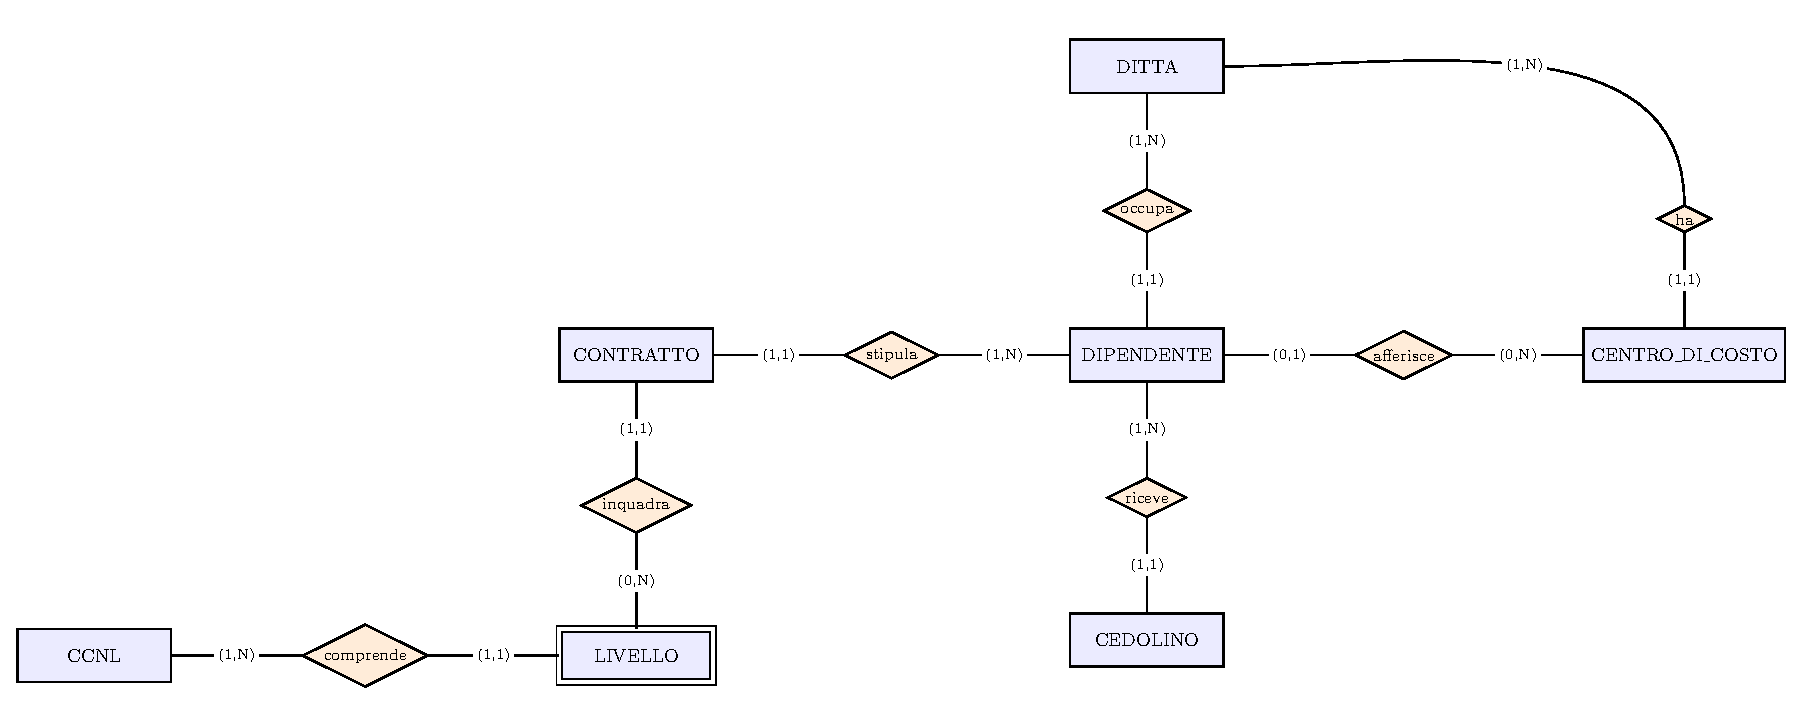
\includegraphics[width=0.72\textwidth]{er-principale}
  \caption{Schema ER semplificato: le entità principali del dominio HR/retributivo.}
  \label{fig:er-principale}
\end{figure}

\begin{figure}[htbp]
  \centering
  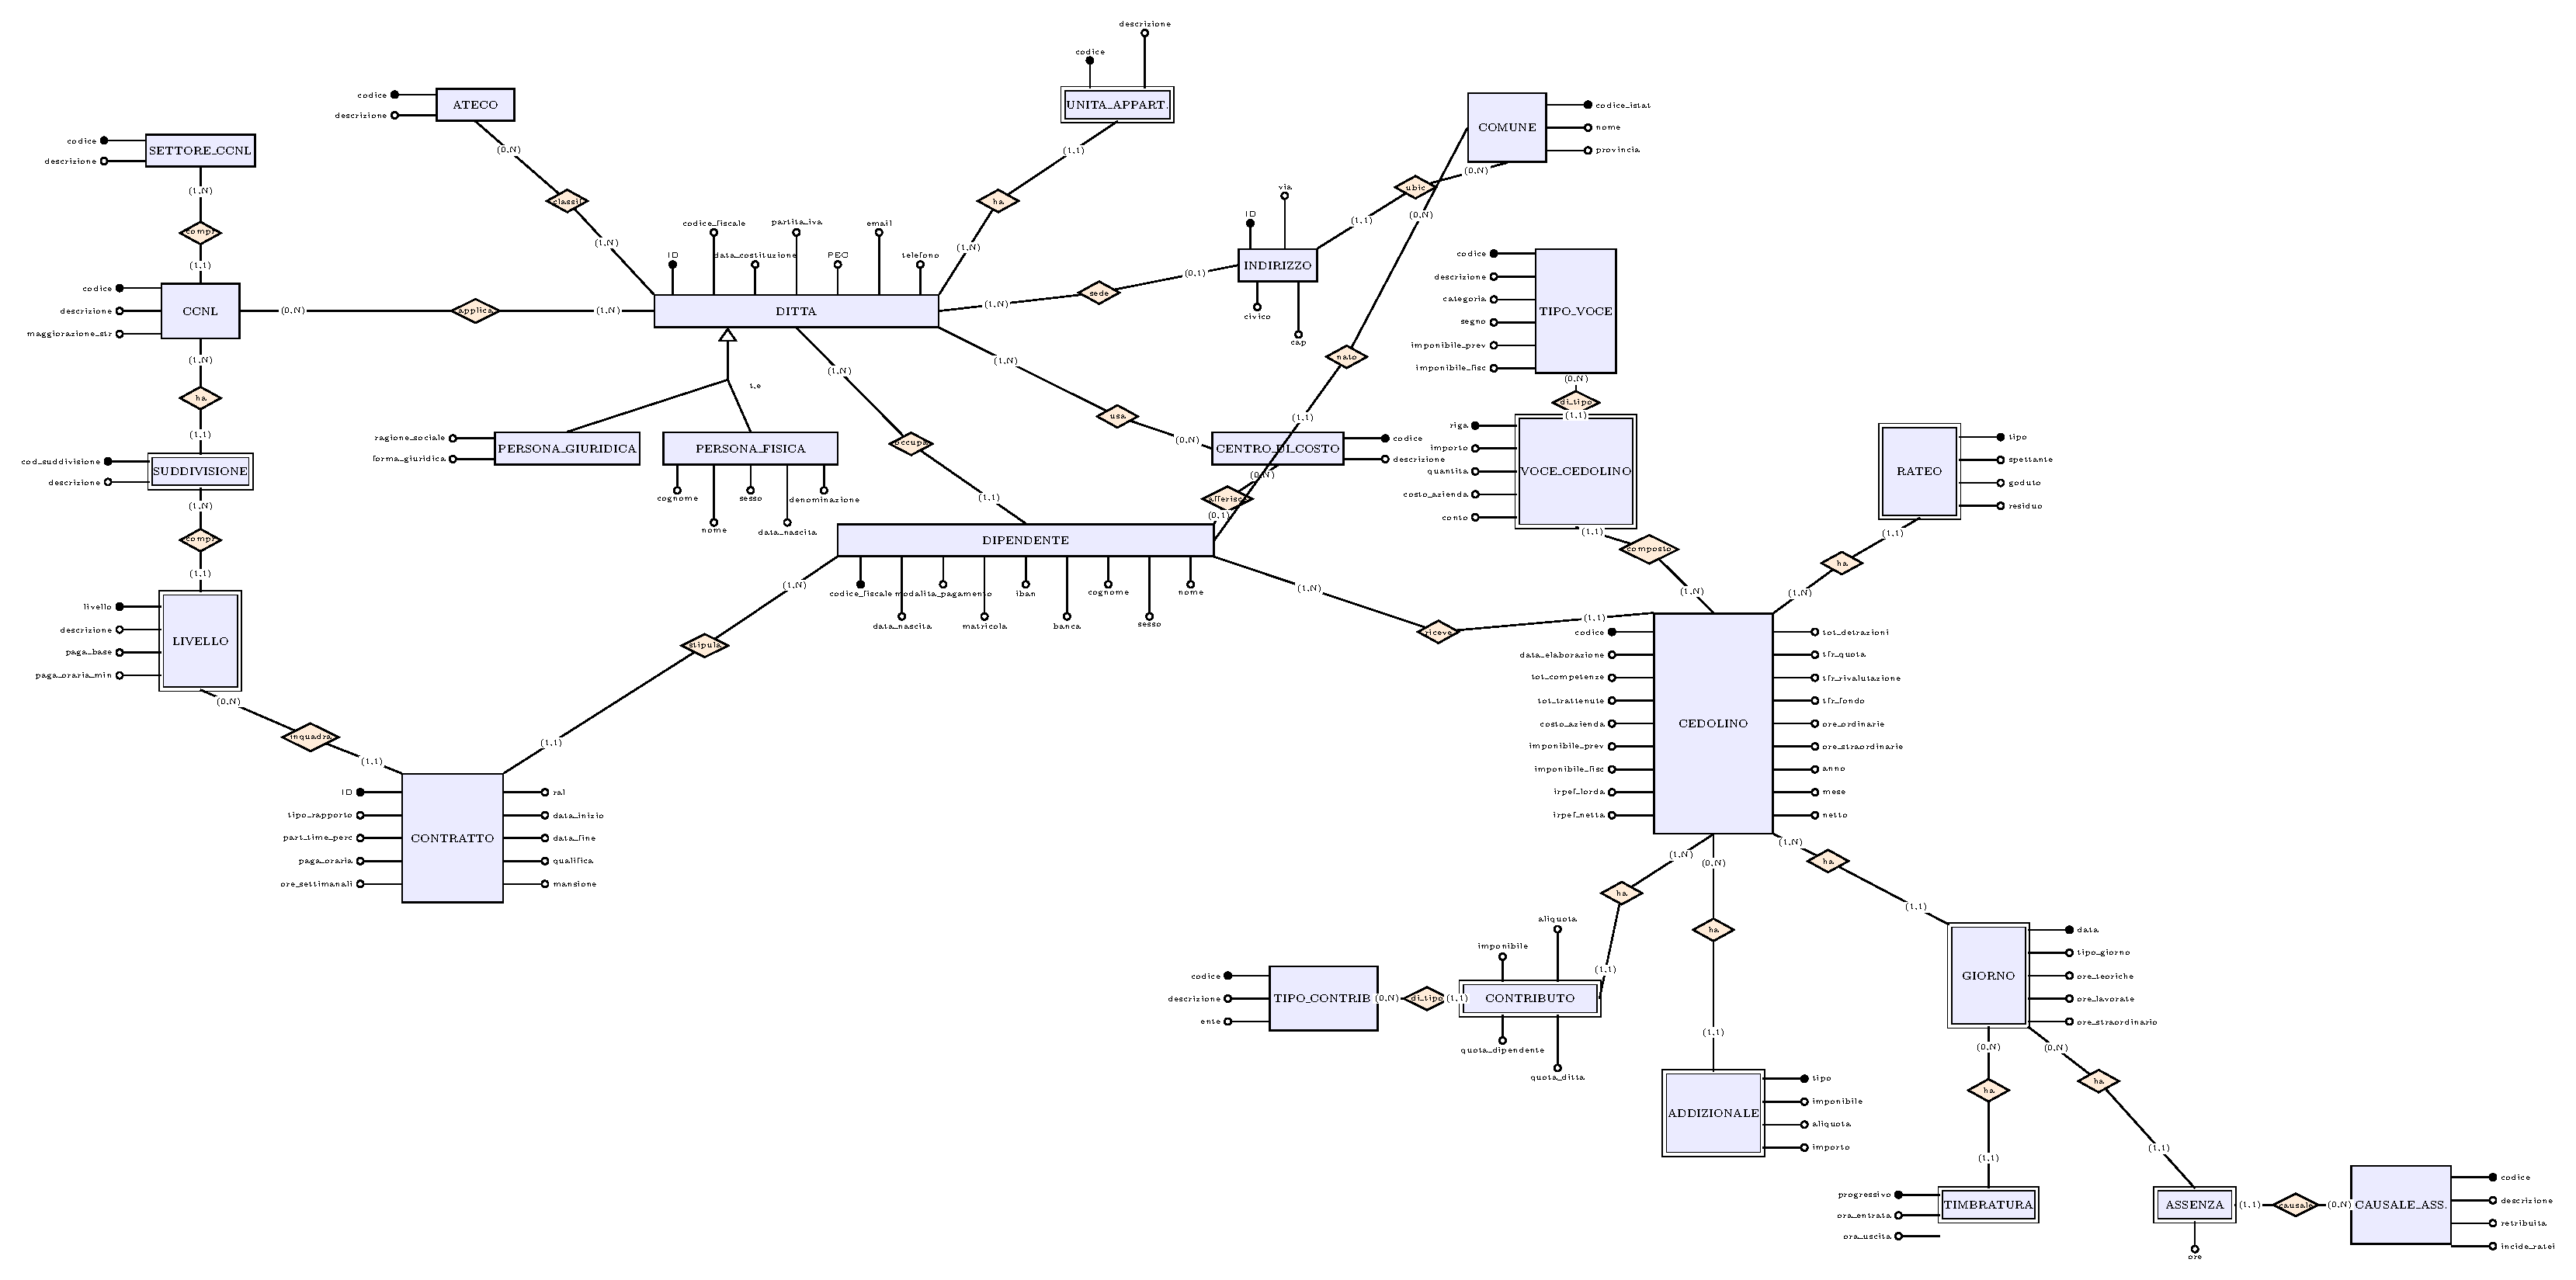
\includegraphics[width=\textwidth]{er-completo}
  \caption{Schema ER completo (${\approx}$25 entità).}
  \label{fig:er-completo}
\end{figure}

\section{Schema logico relazionale (Citus)}
\label{sec:logico-citus}

La traduzione al relazionale distribuito distingue due categorie di tabelle (\Cref{tab:citus-tabelle}):
\textbf{reference table}, cioè i cataloghi condivisi e quasi statici, replicati su ogni nodo per consentire
join locali; e \textbf{tabelle distribuite}, cioè tutto ciò che appartiene al tenant, partizionato per hash
di \texttt{tenant\_id}. Le tabelle distribuite stanno in un \emph{unico gruppo di co-locazione}: un intero
tenant vive su un solo shard, quindi join e transazioni intra-tenant sono \emph{single-node} (nessun 2PC né
traffico di rete). La distribuzione si dichiara con poche primitive:

\begin{lstlisting}[style=sobrio, language=SQL, caption={Dichiarazione della distribuzione in Citus.}, label={lst:ddl-citus}]
-- Cataloghi condivisi: reference table (replicate su ogni nodo)
SELECT create_reference_table('tipo_voce');
-- Tabelle del tenant: distribuite per hash di tenant_id, co-locate tra loro
SELECT create_distributed_table('dipendente', 'tenant_id');
SELECT create_distributed_table('cedolino',   'tenant_id', colocate_with => 'dipendente');
SELECT create_distributed_table('voce_cedolino','tenant_id', colocate_with => 'dipendente');
\end{lstlisting}

\begin{table}[htbp]
  \centering
  \caption{Ripartizione delle tabelle in Citus tra reference (replicate) e distribuite (per \texttt{tenant\_id}).}
  \label{tab:citus-tabelle}
  \begin{tabularx}{\textwidth}{@{}lX@{}}
    \toprule
    \textbf{Tipo} & \textbf{Tabelle} \\
    \midrule
    Reference (replicate su ogni nodo) & comune, ateco, settore\_ccnl, ccnl, suddivisione, livello,
      tipo\_voce, tipo\_contributo, causale\_assenza \\
    Distribuite (hash di \texttt{tenant\_id}, co-locate) & ditta, persona\_giuridica, persona\_fisica,
      indirizzo, centro\_costo, dipendente, contratto, cedolino, voce\_cedolino, rateo, contributo,
      addizionale, timbratura, giorno, assenza, \dots \\
    \bottomrule
  \end{tabularx}
\end{table}

Un vincolo di Citus è che ogni chiave primaria o \texttt{UNIQUE} di una tabella distribuita deve includere la
colonna di distribuzione: la matricola è quindi unica \emph{dentro il tenant}, e il codice fiscale non è
globalmente unico (la stessa persona può lavorare per più ditte). La co-locazione è illustrata in
\Cref{fig:colocazione}.

\begin{figure}[htbp]
  \centering
  \begin{tikzpicture}[font=\footnotesize, node distance=6mm]
    \node[draw, rounded corners, fill=blue!8, minimum width=30mm] (coord) {coordinator (merge/routing)};
    \foreach \i/\x in {1/-4.5, 2/-1.5, 3/1.5, 4/4.5} {
      \node[draw, fill=gray!8, minimum width=20mm, minimum height=13mm, below=12mm of coord, xshift=\x cm] (w\i) {};
      \node[anchor=north] at (w\i.north) {worker \i};
      \node[font=\tiny, align=center] at ([yshift=-2mm]w\i.center) {shard:\\tenant co-locati};
      \draw[-{Latex}] (coord) -- (w\i.north);
    }
  \end{tikzpicture}
  \caption{Co-locazione in Citus: ogni tenant (con tutte le sue tabelle) risiede su un solo shard/worker; il
    coordinator instrada le query single-shard a un worker e fa il merge di quelle cross-shard.}
  \label{fig:colocazione}
\end{figure}

\section{Schema documentale (MongoDB)}
\label{sec:logico-mongo}

Nel modello documentale il cedolino diventa \textbf{un unico documento} che \emph{embedda} tutti i suoi
annidati (\Cref{lst:doc-cedolino}); le collezioni principali sono tre, tutte shardate per \texttt{tenant\_id}
(hashed), mentre i cataloghi restano collezioni non shardate (\Cref{tab:mongo-collezioni}).

\begin{lstlisting}[style=sobrio, language=Java, caption={Documento ``cedolino'': l'aggregato completo in un solo documento (embedding).}, label={lst:doc-cedolino}]
db.cedolini.insertOne({
  tenant_id: 1, cedolino_id: 42, dipendente_id: 7, anno: 2026, mese: 6,
  dipendente:   { sesso: "M", livello: "3", ccnl: "A014", cdc: 1 },
  totali:       { competenze: 2500, trattenute: 700, netto: 1800, costo_azienda: 3300 },
  voci:         [ { riga: 1, tipo: "0201", importo: 2000 }, { riga: 2, tipo: "0301", importo: 500 } ],
  ratei:        [ { tipo: "FERIE", residuo: 2.16 } ],
  contributi:   [ { tipo: "INPS_FPLD", quota_dipendente: 229.75, quota_ditta: 595.25 } ],
  addizionali:  [ { tipo: "REGIONALE", importo: 39.27 } ]
});
\end{lstlisting}

\begin{table}[htbp]
  \centering
  \caption{Collezioni MongoDB e chiave di sharding.}
  \label{tab:mongo-collezioni}
  \begin{tabularx}{\textwidth}{@{}lXl@{}}
    \toprule
    \textbf{Collezione} & \textbf{Contenuto} & \textbf{Shard key} \\
    \midrule
    \texttt{ditte}       & anagrafica della ditta (persona giur./fisica, indirizzi, centri di costo embedded) & \texttt{tenant\_id} (hashed) \\
    \texttt{dipendenti}  & dipendente con i \emph{contratti} embedded & \texttt{tenant\_id} (hashed) \\
    \texttt{cedolini}    & cedolino completo (voci, ratei, contributi, addizionali embedded) & \texttt{tenant\_id} (hashed) \\
    cataloghi            & comuni, ateco, tipi voce/contributo, causali & non shardate \\
    \bottomrule
  \end{tabularx}
\end{table}

La differenza cruciale è nell'\textbf{intestazione del cedolino}: nel relazionale l'anagrafica non si duplica
nel cedolino (si naviga via relazioni), mentre il documentale ne embedda uno \emph{snapshot}. È esattamente
il punto in cui i due modelli divergono e che verrà misurato.

\section{Quando il modello modella bene}
\label{sec:contrasto-modelli}

La suite di test include coppie di operazioni deliberatamente scelte per esporre i punti di forza e di
debolezza dei due modelli:
\begin{itemize}
  \item \textbf{Pro-documentale}: leggere e scrivere il cedolino \emph{completo}. In Mongo è un
        \texttt{findOne}/\texttt{insertOne} su un documento; in Citus è un assemblaggio (o una transazione)
        su sette tabelle co-locate.
  \item \textbf{Pro-relazionale}: modificare un \emph{dato di riferimento} (la categoria di un tipo voce). In
        Citus è \textbf{una riga} su una reference table; in Mongo, con il dato denormalizzato nei cedolini, è
        un \texttt{updateMany} di centinaia di documenti.
\end{itemize}
I risultati di queste coppie sono in \Cref{ch:risultati}.

\section{Evoluzione dello schema}
\label{sec:evoluzione}

Il requisito di gestire l'evoluzione dello schema in corso d'opera (es.\ l'aggiunta di turni e ferie a un
sistema già popolato) evidenzia un'altra divergenza, qui trattata a livello di principio. In
\textbf{Citus/PostgreSQL} un cambiamento strutturale richiede un \texttt{ALTER TABLE} (o nuove tabelle
distribuite) e un \emph{backfill} dei dati: transazionale e verificato dai vincoli, ma con possibili lock e da
propagare a tutti gli shard. In \textbf{MongoDB}, grazie allo schema flessibile, l'aggiunta di campi o array
è quasi gratuita: documenti vecchi e nuovi coesistono e l'assenza dei nuovi campi è gestita dall'applicazione
(schema-on-read). Il documentale è più agile sulle estensioni, il relazionale offre in cambio garanzie di
integrità durante la migrazione.


% 4. Metodologia sperimentale: infrastruttura, deploy, suite di query, misura
\chapter{Metodologia sperimentale}
\label{ch:metodologia}

Le misure sono state condotte su un cluster reale in cloud, con la stessa topologia e lo stesso dataset per i
due sistemi, e con strumenti che rilevano l'impatto \emph{di ciascun nodo}, non solo il tempo visto dal
client. Questo capitolo descrive infrastruttura, deploy, suite di query e strumenti di misura.

\section{Infrastruttura}
\label{sec:infra}

Il cluster è composto da cinque macchine virtuali Azure nella stessa subnet privata (\Cref{tab:vm}). La
scelta di macchine \emph{separate} è deliberata: con client e nodi DB sulla stessa macchina non si vedrebbe
l'impatto della rete e il disco farebbe da collo di bottiglia. La macchina più capace (worker-1, 16 vCPU)
fa da \textbf{coordinator} in Citus e ospita \emph{config server} e \emph{mongos} in MongoDB: è il punto di
merge/instradamento e resta fisso durante lo scaling, così un coordinator potente non maschera il beneficio
di aggiungere worker. I quattro nodi-dati (VM-1\dots VM-4, 4 vCPU ciascuno) sono \textbf{simmetrici}, così lo
scaling è equo. Il traffico interno viaggia sugli IP privati (container in \texttt{network\_mode: host},
niente NAT); le porte DB non sono esposte a internet.

\begin{table}[htbp]
  \centering
  \caption{Topologia del cluster: 5 VM Azure, stessa subnet privata.}
  \label{tab:vm}
  \begin{tabular}{llrrll}
    \toprule
    \textbf{Ruolo} & \textbf{VM (IP priv.)} & \textbf{vCPU} & \textbf{RAM} & \textbf{Citus} & \textbf{MongoDB} \\
    \midrule
    Coordinator & worker-1 (10.0.1.8) & 16 & 32\,GB & coordinator & config server + mongos \\
    Data node   & VM-1 (10.0.1.4)     & 4  & 16\,GB & worker      & shard \\
    Data node   & VM-2 (10.0.1.5)     & 4  & 16\,GB & worker      & shard \\
    Data node   & VM-3 (10.0.1.7)     & 4  & 16\,GB & worker      & shard \\
    Data node   & VM-4 (10.0.1.6)     & 4  & 16\,GB & worker      & shard \\
    \bottomrule
  \end{tabular}
\end{table}

\section{Deploy e gestione dei nodi}
\label{sec:deploy}

Ogni ruolo è impacchettato in un \texttt{docker-compose} dedicato (versioni pinnate: Citus
14.1-alpine, MongoDB 8.3), con autenticazione completa (SCRAM e \texttt{.pgpass} per Citus; keyfile e utente
admin per Mongo). Il deploy porta su i servizi ``nudi'', \emph{non} registrati: l'aggiunta dei nodi al cluster
avviene \textbf{a mano} (\texttt{citus\_add\_node} / \texttt{sh.addShard}), per avere il controllo necessario
agli esperimenti di scaling. Qui emerge una differenza operativa importante: in Citus, dopo aver aggiunto un
worker, la redistribuzione degli shard è \textbf{esplicita} (\texttt{rebalance\_table\_shards}, sincrona); in
MongoDB è affidata al \textbf{balancer automatico}, asincrono e soggetto a soglia. Questa differenza avrà un
peso decisivo sui risultati (\Cref{ch:risultati}).

\begin{lstlisting}[style=sobrio, language=bash, caption={Deploy dei cluster, inizializzazione dello schema e caricamento del dataset (riproducibile).}]
# Deploy dei container (versioni pinnate) su tutte le VM
bash infra/prod/deploy/deploy-citus.sh                 # Citus: coordinator + worker
bash infra/prod/deploy/deploy-mongo.sh                 # Mongo: config server + mongos + shard
# Citus: schema (reference + distribuite) e dati
docker exec -i citus psql -U postgres -d archdata < schema/relational/01_reference.sql
docker exec -i citus psql -U postgres -d archdata < schema/relational/02_distributed.sql
python3 data/genera.py --tenant-count 30 --dip-min 10 --dip-max 25 --seed 42 --out generato
CITUS_CONTAINER=citus bash scripts/carica-citus.sh generato/citus
# MongoDB: cluster a 4 shard pulito + sharding collezioni + caricamento
MONGO_PASSWORD=... bash setup-mongo-4shard.sh
\end{lstlisting}

\section{Suite di query speculare}
\label{sec:suite}

Il confronto equo si basa su una suite di query \textbf{identica nella semantica} sui due sistemi:
\textbf{13 letture} (L01\dots L13) e \textbf{7 scritture} (inserimenti, aggiornamenti, cancellazione), una per
file, con nomi speculari tra la versione SQL (\texttt{.sql}) e quella MongoDB (\texttt{.js}). Le letture vanno
dalla query puntuale single-shard (il cedolino di un dipendente) alle analitiche cross-tenant con percentili e
join ai cataloghi (il gender pay gap mediano per livello). Ogni query è parametrica.

Un accorgimento importante per un test distribuito realistico: nelle \textbf{letture} il carico
\textbf{randomizza} i parametri (tenant, dipendente, mese) a ogni iterazione, così le richieste si distribuiscono
sui vari shard e non colpiscono sempre lo stesso documento; nelle \textbf{scritture} il tenant è invece
\emph{fisso}, per misurare l'effetto della co-locazione (la scrittura di un tenant colpisce un solo nodo).

\section{Strumenti di misura per-nodo}
\label{sec:misura}

Per ogni query si misura la latenza e il throughput sotto \emph{carico sostenuto}, ma soprattutto
\emph{quanto lavora ciascun nodo}. Gli strumenti sono nativi di ciascun sistema:
\begin{itemize}
  \item \textbf{Citus}: il carico è generato con \texttt{pgbench} (connessione persistente); i contatori
        per-nodo (righe elaborate, tempo di esecuzione, letture da cache/disco, WAL) si leggono da
        \texttt{pg\_stat\_statements} propagato a tutti i nodi con \texttt{run\_command\_on\_all\_nodes()},
        con azzeramento e delta attorno a ogni misura.
  \item \textbf{MongoDB}: il carico è un ciclo \texttt{mongosh}; i contatori per-shard vengono da
        \texttt{serverStatus().opcounters}, l'uso di CPU/RAM da \texttt{docker stats} campionato su ogni nodo.
  \item \textbf{Sistema operativo}: CPU, RAM e I/O di disco per nodo si campionano da \texttt{/proc} durante
        ogni run, raccogliendo tutto in CSV strutturati (fonte dei grafici e delle tabelle del
        \Cref{ch:risultati}).
\end{itemize}

Due note metodologiche. Le query si eseguono \emph{una alla volta}, senza accesso concorrente, così l'impatto
è attribuibile alla singola query e leggibile su ogni nodo. E la relazione \textbf{cache/disco}: a scala
piccola il dataset entra tutto in RAM, quindi le letture non toccano il disco (\texttt{blk\_read}${=}0$); le
letture fisiche da disco compaiono solo quando i dati superano la RAM, cioè nell'esperimento a dati crescenti,
ed è lì che il disco diventa il collo di bottiglia. Per questo lo scaling per nodi si misura a freddo (cache
svuotata) e quello a dati crescenti a caldo (per vedere la capacità massima e il punto in cui la cache cede).


% 5. Risultati e analisi: scalabilita' nodi/dati, scritture, guasti; Citus vs Mongo
%    (il cuore: tabelle, grafici, confronti)
\chapter{Risultati e analisi}
\label{ch:risultati}

Questo capitolo raccoglie le misure dei test e le analizza. Salvo diverso avviso i numeri sono medie su tre esecuzioni
a freddo, ovvero la cache viene svuotata prima di ogni esecuzione, per lo scaling per nodi, e misure a caldo per lo scaling sui dati. 
Il dataset di partenza è delle stesse dimensioni su entrambi i sistemi (30 ditte, 554 dipendenti), generato con lo script dedicato.

\section{Baseline in lettura e i due regimi}
\label{sec:baseline}

Su Citus a un nodo, sotto carico sostenuto, emergono due regimi netti. Le query \textbf{single-shard} (cedolino singolo, cedolini di una ditta, riepiloghi per un tenant) stanno a \textbf{1--3\,ms} con throughput
fino a ${\sim}680$ op/s: colpiscono un solo shard e il coordinator ha solo un overhead fisso di instradamento. Le analitiche \textbf{cross-shard} (percentili, aggregazioni cross-tenant, spesa per categoria)
stanno a \textbf{55--85\,ms} con 13--18 op/s: ogni worker satura la CPU per lo scan (100--190\,\%, multi-core)
e il coordinator (${\sim}40\,\%$) fa il merge. Questa distinzione tra i due regimi si ritrova in tutti gli esperimenti seguenti.

\section{Scalabilità per numero di nodi (Citus)}
\label{sec:scaling-nodi}

A parità di dati si passa da 1 a 4 nodi, ridistribuendo gli shard a ogni passo. Le query cross-shard scalano
in modo \textbf{quasi lineare} (\Cref{tab:scaling-nodi,fig:scaling-nodi}): con 4 nodi lo speedup è
\textbf{3.8--4.6$\times$}. Le single-shard restano invece piatte: colpiscono un solo shard su un solo nodo,
quindi aggiungere worker non le tocca (ma sono già velocissime). Il lavoro si distribuisce: la CPU e il tempo
di esecuzione \emph{per worker} calano proporzionalmente (per L04, la CPU del worker passa da 142\,\% a 24\,\%
e le righe per worker si dimezzano a ogni raddoppio).

\begin{table}[htbp]
  \centering
  \caption{Latenza (ms) al crescere dei nodi e speedup 1$\to$4. Cross-shard vs single-shard.}
  \label{tab:scaling-nodi}
  \begin{tabular}{lrrrrr}
    \toprule
    \textbf{Query} & \textbf{1 nodo} & \textbf{2 nodi} & \textbf{3 nodi} & \textbf{4 nodi} & \textbf{speedup} \\
    \midrule
    L04 gender gap mediano & 71.9 & 45.0 & 23.2 & 18.3 & \textbf{3.9$\times$} \\
    L05 top-N retribuzioni & 65.8 & 33.7 & 19.4 & 14.9 & \textbf{4.4$\times$} \\
    L06 assenteismo/mese   & 61.4 & 31.2 & 19.9 & 15.4 & \textbf{4.0$\times$} \\
    L08 trend costo lavoro & 56.1 & 24.0 & 15.9 & 12.1 & \textbf{4.6$\times$} \\
    L11 spesa/categoria    & 75.6 & 52.7 & 25.3 & 20.1 & \textbf{3.8$\times$} \\
    L12 ferie residue      & 75.4 & 59.7 & 25.2 & 19.5 & \textbf{3.9$\times$} \\
    \midrule
    L01 cedolino singolo \emph{(single-shard)} & 1.5 & 1.5 & 1.5 & 1.5 & 1.0$\times$ \\
    \bottomrule
  \end{tabular}
\end{table}

Il dettaglio completo di \emph{tutte} le metriche raccolte (latenza, throughput, CPU per worker, tempo di
esecuzione e righe elaborate per worker) per ognuna delle 13 query è in \Cref{tab:scaling-nodi-full}: mostra
esplicitamente come, all'aumentare dei nodi, il lavoro \emph{per worker} (CPU, \texttt{exec}, righe) si
riduca, mentre l'overhead sul coordinator resta pressoché costante.

\begingroup
\footnotesize
\begin{longtable}{@{}llrrrr@{}}
\caption{Scalabilità per numero di nodi (Citus): tutte le metriche raccolte, per le 13 query, a 1--4 nodi. Le metriche per-worker sono la media sui worker attivi.}\label{tab:scaling-nodi-full}\\
\toprule \textbf{Query} & \textbf{Parametro} & \textbf{1 nodo} & \textbf{2 nodi} & \textbf{3 nodi} & \textbf{4 nodi} \\ \midrule \endfirsthead
\toprule \textbf{Query} & \textbf{Parametro} & \textbf{1 nodo} & \textbf{2 nodi} & \textbf{3 nodi} & \textbf{4 nodi} \\ \midrule \endhead
\multirow{5}{*}{L01 cedolino singolo} & latenza (ms)     & 1.5 & 1.5 & 1.5 & 1.5 \\
 & throughput (op/s) & 680 & 666 & 669 & 688 \\
 & CPU worker (\%)   & 11 & 6 & 4 & 3 \\
 & exec worker (ms)  & 138 & 63 & 47 & 34 \\
 & righe/worker      & 6797 & 3331 & 2230 & 1718 \\ \midrule
\multirow{5}{*}{L02 cedolini ditta/periodo} & latenza (ms)     & 1.5 & 1.6 & 1.6 & 1.5 \\
 & throughput (op/s) & 669 & 636 & 638 & 654 \\
 & CPU worker (\%)   & 15 & 7 & 5 & 4 \\
 & exec worker (ms)  & 171 & 82 & 56 & 43 \\
 & righe/worker      & 6699 & 3182 & 2127 & 1636 \\ \midrule
\multirow{5}{*}{L03 costo per centro} & latenza (ms)     & 2.3 & 2.3 & 2.3 & 2.3 \\
 & throughput (op/s) & 438 & 431 & 437 & 433 \\
 & CPU worker (\%)   & 27 & 14 & 9 & 7 \\
 & exec worker (ms)  & 646 & 315 & 213 & 161 \\
 & righe/worker      & 210192 & 103456 & 69909 & 51988 \\ \midrule
\multirow{5}{*}{L04 gender gap mediano} & latenza (ms)     & 71.9 & 45.0 & 23.2 & 18.3 \\
 & throughput (op/s) & 14 & 23 & 43 & 55 \\
 & CPU worker (\%)   & 142 & 57 & 26 & 24 \\
 & exec worker (ms)  & 531 & 335 & 367 & 347 \\
 & righe/worker      & 77375 & 63064 & 79899 & 75667 \\ \midrule
\multirow{5}{*}{L05 top-N retribuzioni} & latenza (ms)     & 65.8 & 33.7 & 19.4 & 14.9 \\
 & throughput (op/s) & 15 & 31 & 52 & 67 \\
 & CPU worker (\%)   & 129 & 33 & 20 & 20 \\
 & exec worker (ms)  & 327 & 237 & 244 & 266 \\
 & righe/worker      & 54840 & 55080 & 61960 & 60240 \\ \midrule
\multirow{5}{*}{L06 assenteismo per mese} & latenza (ms)     & 61.4 & 31.2 & 19.9 & 15.4 \\
 & throughput (op/s) & 16 & 32 & 50 & 65 \\
 & CPU worker (\%)   & 122 & 30 & 21 & 17 \\
 & exec worker (ms)  & 1700 & 1225 & 1224 & 923 \\
 & righe/worker      & 245000 & 242750 & 251667 & 187125 \\ \midrule
\multirow{5}{*}{L07 straordinari per centro} & latenza (ms)     & 3.1 & 3.1 & 3.1 & 3.2 \\
 & throughput (op/s) & 321 & 322 & 326 & 317 \\
 & CPU worker (\%)   & 41 & 21 & 14 & 11 \\
 & exec worker (ms)  & 1631 & 889 & 603 & 441 \\
 & righe/worker      & 12843 & 6435 & 4343 & 3165 \\ \midrule
\multirow{5}{*}{L08 trend costo lavoro} & latenza (ms)     & 56.1 & 24.0 & 15.9 & 12.1 \\
 & throughput (op/s) & 18 & 42 & 63 & 82 \\
 & CPU worker (\%)   & 106 & 14 & 12 & 12 \\
 & exec worker (ms)  & 466 & 368 & 360 & 351 \\
 & righe/worker      & 42880 & 50080 & 50267 & 49500 \\ \midrule
\multirow{5}{*}{L09 organico per livello} & latenza (ms)     & 57.7 & 24.5 & 17.0 & 12.8 \\
 & throughput (op/s) & 17 & 41 & 59 & 78 \\
 & CPU worker (\%)   & 106 & 15 & 14 & 13 \\
 & exec worker (ms)  & 186 & 134 & 127 & 125 \\
 & righe/worker      & 51852 & 60991 & 58640 & 58234 \\ \midrule
\multirow{5}{*}{L10 cedolino completo} & latenza (ms)     & 82.7 & 63.3 & 27.9 & 21.7 \\
 & throughput (op/s) & 12 & 16 & 36 & 46 \\
 & CPU worker (\%)   & 189 & 91 & 33 & 31 \\
 & exec worker (ms)  & 169 & 97 & 116 & 112 \\
 & righe/worker      & 121 & 79 & 120 & 115 \\ \midrule
\multirow{5}{*}{L11 spesa per categoria} & latenza (ms)     & 75.6 & 52.7 & 25.3 & 20.1 \\
 & throughput (op/s) & 13 & 19 & 40 & 50 \\
 & CPU worker (\%)   & 154 & 68 & 27 & 25 \\
 & exec worker (ms)  & 1464 & 535 & 524 & 543 \\
 & righe/worker      & 73497 & 52907 & 73066 & 69158 \\ \midrule
\multirow{5}{*}{L12 ferie residue} & latenza (ms)     & 75.4 & 59.7 & 25.2 & 19.5 \\
 & throughput (op/s) & 13 & 17 & 40 & 51 \\
 & CPU worker (\%)   & 165 & 82 & 32 & 30 \\
 & exec worker (ms)  & 909 & 439 & 545 & 528 \\
 & righe/worker      & 3990 & 2520 & 3963 & 3842 \\ \midrule
\multirow{5}{*}{L13 riepilogo assenze} & latenza (ms)     & 3.4 & 3.5 & 3.5 & 3.4 \\
 & throughput (op/s) & 291 & 290 & 289 & 291 \\
 & CPU worker (\%)   & 38 & 19 & 12 & 10 \\
 & exec worker (ms)  & 923 & 453 & 305 & 230 \\
 & righe/worker      & 29320 & 14487 & 9628 & 7281 \\ \midrule
\bottomrule
\end{longtable}
\endgroup


\begin{figure}[htbp]
  \centering
  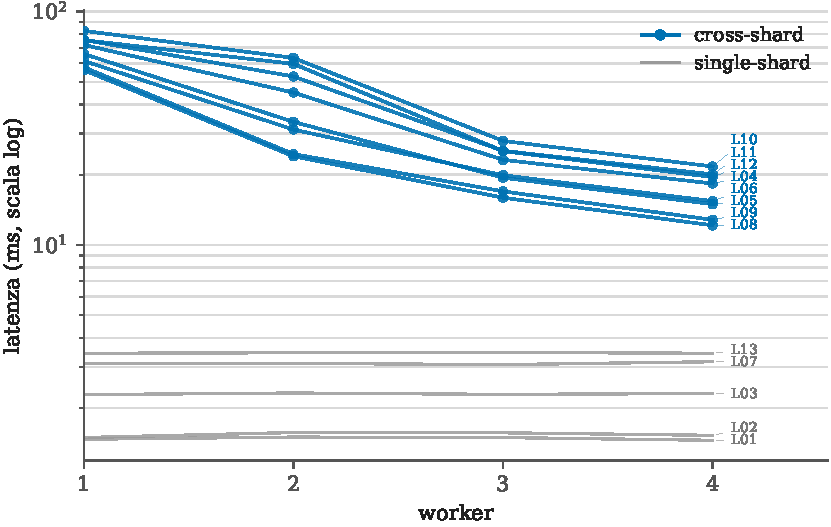
\includegraphics[width=0.82\textwidth]{fig-scaling-nodi-citus}
  \caption{Citus, scaling per nodi (tutte le 13 letture, scala log; codice query in coda a ogni linea): le
    cross-shard calano nettamente al crescere dei nodi, le single-shard restano piatte.}
  \label{fig:scaling-nodi}
\end{figure}

\begin{lstlisting}[style=sobrio, language=bash, caption={Esecuzione: aggiunta di un worker e rebalance, poi 3 run a freddo delle 13 letture e media (ripetuto a 1, 2, 3, 4 nodi).}]
bash citus-add-node.sh 10.0.1.5 && bash citus-rebalance.sh       # ad ogni passo di scaling
for i in 1 2 3; do bash azzera-cache-citus.sh; \
  bash esegui-suite-citus.sh 10 queries/relational/letture/*.sql; done
bash media-citus.sh
\end{lstlisting}

\section{Scalabilità per volume di dati (Citus)}
\label{sec:scaling-dati}

A numero di nodi fisso (4) si aumenta il volume dei dati. Le cross-shard \textbf{degradano in modo
super-lineare} (\Cref{tab:scaling-dati,fig:scaling-dati}): da 30 a 480 ditte L11 passa da 20 a 114\,ms
(5.7$\times$), con un salto netto tra 240 e 480 ditte. Le single-shard restano \textbf{piatte} (${\sim}1.5$\,ms
a ogni scala): indicizzate e mirate a un tenant, sono insensibili al volume globale, che è il vantaggio del
multitenant co-locato. Le letture da disco (\texttt{blk\_read}) restano nulle: a questa scala i dati stanno
ancora in RAM, quindi il degrado è \emph{CPU-bound} (più righe da scandire in cache). L'esperimento si è
fermato a 480 ditte perché a quel punto la tendenza era già chiara e il carico risultava distribuito su tutti
i nodi: proseguire non avrebbe aggiunto informazione.

\begin{table}[htbp]
  \centering
  \caption{Latenza (ms) al crescere dei dati, a 4 nodi fissi.}
  \label{tab:scaling-dati}
  \begin{tabular}{lrrrr}
    \toprule
    \textbf{Ditte} & \textbf{L01 single-shard} & \textbf{L04 gender gap} & \textbf{L06 assenteismo} & \textbf{L11 spesa} \\
    \midrule
    30 (base) & 1.5 & 18.3 & 15.4 & 20.1 \\
    60        & 1.5 & 20.4 & 17.5 & 24.6 \\
    120       & 1.5 & 24.0 & 25.1 & 34.9 \\
    240       & 1.4 & 30.9 & 51.2 & 66.0 \\
    480       & 1.6 & \textbf{68.3} & \textbf{73.1} & \textbf{114.1} \\
    \bottomrule
  \end{tabular}
\end{table}

Il dettaglio completo di tutte le metriche per le 13 query, a ogni scala, è in \Cref{tab:scaling-dati-full}:
si vede come il tempo di esecuzione e le righe elaborate per worker crescano col volume, mentre le query
single-shard restano invariate.

\begingroup
\footnotesize
\begin{longtable}{@{}llrrrrr@{}}
\caption{Scalabilità per volume di dati (Citus, 4 nodi fissi): tutte le metriche per le 13 query, da 30 a 480 ditte.}\label{tab:scaling-dati-full}\\
\toprule \textbf{Query} & \textbf{Parametro} & \textbf{30} & \textbf{60} & \textbf{120} & \textbf{240} & \textbf{480} \\* \midrule \endfirsthead
\toprule \textbf{Query} & \textbf{Parametro} & \textbf{30} & \textbf{60} & \textbf{120} & \textbf{240} & \textbf{480} \\* \midrule \endhead
\multirow{5}{*}{L01 cedolino singolo} & latenza (ms)     & 1.5 & 1.5 & 1.5 & 1.4 & 1.6 \\
 & throughput (op/s) & 688 & 659 & 655 & 705 & 643 \\
 & CPU worker (\%)   & 3 & 6 & 6 & 5 & 4 \\
 & exec worker (ms)  & 34 & 36 & 36 & 38 & 34 \\
 & righe/worker      & 1718 & 1647 & 1636 & 1762 & 1607 \\ \midrule
\multirow{5}{*}{L02 cedolini ditta/periodo} & latenza (ms)     & 1.5 & 1.5 & 1.5 & 1.6 & 1.5 \\
 & throughput (op/s) & 654 & 659 & 674 & 635 & 682 \\
 & CPU worker (\%)   & 4 & 5 & 4 & 4 & 4 \\
 & exec worker (ms)  & 43 & 44 & 45 & 33 & 36 \\
 & righe/worker      & 1636 & 1648 & 1684 & 1588 & 1706 \\ \midrule
\multirow{5}{*}{L03 costo per centro} & latenza (ms)     & 2.3 & 2.3 & 2.4 & 2.4 & 2.4 \\
 & throughput (op/s) & 433 & 438 & 424 & 414 & 423 \\
 & CPU worker (\%)   & 7 & 7 & 7 & 8 & 8 \\
 & exec worker (ms)  & 161 & 164 & 171 & 175 & 185 \\
 & righe/worker      & 51988 & 52548 & 50820 & 49680 & 50748 \\ \midrule
\multirow{5}{*}{L04 gender gap mediano} & latenza (ms)     & 18.3 & 20.4 & 24.0 & 30.9 & 68.3 \\
 & throughput (op/s) & 55 & 49 & 42 & 32 & 15 \\
 & CPU worker (\%)   & 24 & 26 & 26 & 28 & 38 \\
 & exec worker (ms)  & 347 & 623 & 947 & 1430 & 1325 \\
 & righe/worker      & 75667 & 164762 & 283664 & 454734 & 411049 \\ \midrule
\multirow{5}{*}{L05 top-N retribuzioni} & latenza (ms)     & 14.9 & 14.8 & 15.8 & 15.7 & 17.4 \\
 & throughput (op/s) & 67 & 68 & 63 & 64 & 58 \\
 & CPU worker (\%)   & 20 & 22 & 23 & 27 & 30 \\
 & exec worker (ms)  & 266 & 423 & 587 & 953 & 1475 \\
 & righe/worker      & 60240 & 89401 & 98425 & 102080 & 92320 \\ \midrule
\multirow{5}{*}{L06 assenteismo per mese} & latenza (ms)     & 15.4 & 17.5 & 25.1 & 51.2 & 73.1 \\
 & throughput (op/s) & 65 & 57 & 40 & 20 & 14 \\
 & CPU worker (\%)   & 17 & 32 & 39 & 68 & 91 \\
 & exec worker (ms)  & 923 & 2445 & 3337 & 3655 & 5274 \\
 & righe/worker      & 187125 & 326326 & 262342 & 134554 & 94256 \\ \midrule
\multirow{5}{*}{L07 straordinari per centro} & latenza (ms)     & 3.2 & 3.2 & 3.2 & 3.2 & 3.3 \\
 & throughput (op/s) & 317 & 317 & 309 & 312 & 307 \\
 & CPU worker (\%)   & 11 & 11 & 11 & 11 & 12 \\
 & exec worker (ms)  & 441 & 478 & 474 & 483 & 480 \\
 & righe/worker      & 3165 & 3173 & 3093 & 3122 & 3068 \\ \midrule
\multirow{5}{*}{L08 trend costo lavoro} & latenza (ms)     & 12.1 & 12.6 & 13.9 & 14.9 & 17.8 \\
 & throughput (op/s) & 82 & 79 & 72 & 67 & 56 \\
 & CPU worker (\%)   & 12 & 14 & 18 & 27 & 39 \\
 & exec worker (ms)  & 351 & 673 & 1148 & 2091 & 3460 \\
 & righe/worker      & 49500 & 68904 & 66960 & 64608 & 54144 \\ \midrule
\multirow{5}{*}{L09 organico per livello} & latenza (ms)     & 12.8 & 13.5 & 14.6 & 16.8 & 20.2 \\
 & throughput (op/s) & 78 & 74 & 69 & 60 & 49 \\
 & CPU worker (\%)   & 13 & 13 & 14 & 15 & 17 \\
 & exec worker (ms)  & 125 & 210 & 336 & 546 & 881 \\
 & righe/worker      & 58234 & 104710 & 185220 & 321186 & 535095 \\ \midrule
\multirow{5}{*}{L10 cedolino completo} & latenza (ms)     & 21.7 & 21.7 & 21.8 & 21.3 & 21.7 \\
 & throughput (op/s) & 46 & 46 & 46 & 47 & 46 \\
 & CPU worker (\%)   & 31 & 32 & 31 & 31 & 30 \\
 & exec worker (ms)  & 112 & 115 & 115 & 119 & 116 \\
 & righe/worker      & 115 & 115 & 115 & 118 & 115 \\ \midrule
\multirow{5}{*}{L11 spesa per categoria} & latenza (ms)     & 20.1 & 24.6 & 34.9 & 66.0 & 114.1 \\
 & throughput (op/s) & 50 & 41 & 29 & 15 & 9 \\
 & CPU worker (\%)   & 25 & 27 & 29 & 42 & 52 \\
 & exec worker (ms)  & 543 & 1102 & 1292 & 1404 & 1718 \\
 & righe/worker      & 69158 & 136854 & 195912 & 213332 & 246070 \\ \midrule
\multirow{5}{*}{L12 ferie residue} & latenza (ms)     & 19.5 & 20.4 & 23.5 & 28.3 & 49.6 \\
 & throughput (op/s) & 51 & 49 & 43 & 35 & 20 \\
 & CPU worker (\%)   & 30 & 35 & 38 & 44 & 65 \\
 & exec worker (ms)  & 528 & 1007 & 1576 & 2569 & 3100 \\
 & righe/worker      & 3842 & 7365 & 12780 & 21240 & 24240 \\ \midrule
\multirow{5}{*}{L13 riepilogo assenze} & latenza (ms)     & 3.4 & 3.6 & 3.6 & 3.6 & 3.5 \\
 & throughput (op/s) & 291 & 279 & 276 & 280 & 289 \\
 & CPU worker (\%)   & 10 & 10 & 10 & 10 & 10 \\
 & exec worker (ms)  & 230 & 233 & 224 & 228 & 193 \\
 & righe/worker      & 7281 & 6978 & 6895 & 7010 & 7220 \\ \midrule
\bottomrule
\end{longtable}
\endgroup


\begin{figure}[htbp]
  \centering
  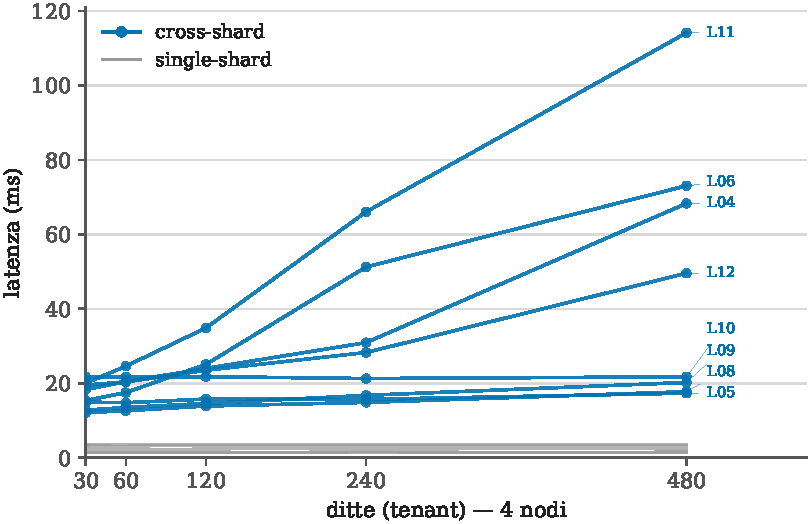
\includegraphics[width=0.82\textwidth]{fig-scaling-dati-citus}
  \caption{Citus, scaling per dati (tutte le 13 letture, 4 nodi fissi): degrado super-lineare delle
    cross-shard; single-shard insensibili al volume.}
  \label{fig:scaling-dati}
\end{figure}

\begin{lstlisting}[style=sobrio, language=bash, caption={Esecuzione: a 4 nodi fissi, un lotto per volta genera nuovi tenant, carica e misura a caldo (ripetuto fino a 480 ditte).}]
bash scala-dati-citus.sh 31 30 60ditte      # +30 tenant -> 60 ditte; poi 61 60 120ditte; ...
\end{lstlisting}

\section{Scritture distribuite (Citus)}
\label{sec:scritture-citus}

Le scritture, misurate a 4 nodi (\Cref{tab:scritture-citus}), mostrano l'effetto della \textbf{co-locazione}:
\textbf{cinque scritture su sei colpiscono un solo nodo} (quello dello shard del tenant), mentre gli altri tre
worker restano inattivi. La scrittura di un singolo tenant \emph{non si distribuisce} aggiungendo nodi; il
throughput aggregato scala solo distribuendo scritture su tenant diversi. Il costo cresce con le righe/tabelle
toccate e il WAL prodotto: dalla semplice \texttt{UPDATE} (U02, 605 op/s) alla \textbf{transazione}
multi-tabella I03 (17 op/s, ${\sim}1$\,MB di WAL) c'è un fattore ${\sim}35\times$. L'unica scrittura che tocca
\textbf{tutti i nodi} è U03, l'aggiornamento di un dato di riferimento su una reference table (replicata
ovunque): una riga logica, ma applicata su ogni nodo.

\begin{table}[htbp]
  \centering
  \caption{Scritture a 4 nodi (N${=}300$ operazioni per query).}
  \label{tab:scritture-citus}
  \begin{tabular}{llrrl}
    \toprule
    \textbf{Op.} & \textbf{Descrizione} & \textbf{lat (ms/op)} & \textbf{tps} & \textbf{dove scrive} \\
    \midrule
    U02 & licenziamento (update 1 riga)     & 1.7  & 605 & solo 1 nodo \\
    U01 & coordinate bancarie               & 3.7  & 273 & solo 1 nodo \\
    U04 & update concorrente (riga cond.)   & 3.8  & 266 & solo 1 nodo \\
    I01 & inserimento timbratura            & 10.6 & 94  & solo 1 nodo \\
    U03 & modifica dato di riferimento      & 21.1 & 47  & \textbf{tutti i nodi} \\
    I03 & elaborazione cedolino (transazione)& 57.4 & 17  & solo 1 nodo \\
    \bottomrule
  \end{tabular}
\end{table}

\begin{lstlisting}[style=sobrio, language=bash, caption={Esecuzione delle scritture (Citus): N${=}300$ ripetizioni per query, tenant fisso.}]
bash esegui-scritture-citus.sh 300 queries/relational/scritture/*.sql
\end{lstlisting}

\section{Comportamento in presenza di guasti (Citus)}
\label{sec:guasti-citus}

Il comportamento \textbf{CP} è stato messo alla prova eseguendo una query cross-shard (L04) in un ciclo mentre
un worker scelto a caso viene spento e poi riacceso (11 prove). Il risultato è netto e coerente: spegnendo
\emph{qualsiasi} worker, la query fallisce per \textbf{tutta} la finestra di down (15\,s), perché ha bisogno
degli shard di ogni nodo, quindi manca sempre qualcosa e \textbf{non restituisce risultati parziali} (le righe
crollano da $N$ a $0$). L'error-rate medio è ${\sim}51\,\%$, il recupero è \textbf{automatico e rapido}
(prima risposta ${\sim}0.5$\,s dopo il riavvio del container). I quattro worker danno lo stesso error-rate:
ognuno è essenziale, nessuno ridondante (copia singola, \texttt{shard\_replication\_factor}${=}1$). È la
consistenza scelta al posto della disponibilità.

\begin{lstlisting}[style=sobrio, language=bash, caption={Esecuzione del test di guasto (Citus): L04 in loop mentre un worker a caso viene spento (10--25\,s) e riacceso, su 45\,s totali.}]
bash test-guasto-citus.sh queries/relational/letture/L04_gender_gap_mediano.sql random 10 15 45
\end{lstlisting}

\section{MongoDB}
\label{sec:mongo}

\subsection{Scalabilità per shard: il balancer non distribuisce a scala piccola}
Sul cluster documentale il regime ``più shard, stessi dati'' ha rivelato un comportamento che è esso stesso il
risultato più interessante. Con il dataset base (\texttt{cedolini} ${\approx}42$\,MB), il balancer di MongoDB
\textbf{non distribuisce}: con la dimensione di range di default (128\,MB) la soglia di migrazione è 384\,MB,
mai raggiunta, quindi resta un solo chunk su un solo shard. Anche forzando le condizioni, con il range
ridotto a 4\,MB (soglia 12\,MB) e uno \emph{split manuale} in 10 chunk, il balancer, pur attivo (\texttt{mode: full},
888 round eseguiti), \textbf{non ha migrato nulla}. Di conseguenza il secondo shard resta inattivo (0.2\,\%
CPU) e le prestazioni a 1 e 2 shard sono \textbf{identiche} (\Cref{tab:mongo-shard}): aggiungere shard non
porta alcun beneficio. È l'opposto di Citus, dove il rebalance esplicito distribuisce sempre. Il balancer
distribuisce solo a \emph{volume grande}: già a ${\approx}230$ ditte (cedolini ${>}300$\,MB) inizia a spargere
i chunk sugli shard, e il comportamento dipende dunque dalla scala.

\begin{table}[htbp]
  \centering
  \caption{MongoDB, latenza (ms) a 1 e 2 shard: identica, perché il 2\textsuperscript{o} shard resta inattivo.}
  \label{tab:mongo-shard}
  \begin{tabular}{lrr}
    \toprule
    \textbf{Query} & \textbf{1 shard} & \textbf{2 shard} \\
    \midrule
    L04 gender gap (aggregazione) & 7.2  & 7.2  \\
    L11 spesa per categoria        & 12.4 & 12.5 \\
    L01 cedolino singolo (mirata)  & 2.3  & 2.3  \\
    \bottomrule
  \end{tabular}
\end{table}

\begin{lstlisting}[style=sobrio, language=bash, caption={Esecuzione dello scaling per shard (MongoDB): aggiunta automatica degli shard e 3 run a freddo delle letture per passo.}]
export MONGO_PASSWORD=...
bash scala-nodi-mongo.sh 4        # dal numero di shard attuale fino a 4
\end{lstlisting}

\subsection{Scalabilità per volume di dati (MongoDB)}
\label{sec:mongo-dati}
Applicando lo \emph{stesso} protocollo delle controparti Citus (identica suite, misura a caldo, carico
randomizzato, contatori per shard), a numero di shard fisso (4) si aumenta il volume dei dati. Qui si completa
il quadro emerso con lo scaling per shard: mentre a scala piccola il balancer non distribuiva, \textbf{a volume
grande distribuisce davvero}. A ogni scala i
\texttt{cedolini} risultano spartiti su \textbf{tutti e 4 gli shard}, attivi al 48--65\,\% di CPU. Le query
cross-shard degradano super-linearmente (\Cref{tab:mongo-dati}): L04 26$\to$185\,ms, L11 34$\to$308\,ms; le
più pesanti, L06 e L12, crescono a dismisura (302$\to$2834\,ms e 476$\to$4786\,ms) perché aggregano tutti i cedolini
scorrendone gli array annidati: a scala grande il costo dell'embedding sull'intera collezione diventa
dominante. Le query mirate restano piatte (L01 ${\sim}2.6$\,ms).

\begin{table}[htbp]
  \centering
  \caption{MongoDB, scalabilità per dati (4 shard fissi): latenza (ms) al crescere del volume.}
  \label{tab:mongo-dati}
  \begin{tabular}{rrrrrr}
    \toprule
    \textbf{Ditte} & \textbf{L01} & \textbf{L04} & \textbf{L11} & \textbf{L06} & \textbf{L12} \\
    \midrule
     230 & 2.6 & 26.0  & 34.2  & 301.6  & 476.2  \\
     630 & 2.6 & 61.6  & 80.0  & 729.1  & 1174.1 \\
    1430 & 2.7 & 122.2 & 178.0 & 1684.9 & 2759.5 \\
    2630 & 2.7 & 185.2 & 308.0 & 2833.8 & 4786.3 \\
    \bottomrule
  \end{tabular}
\end{table}

Il dettaglio completo per tutte le 13 query e tutte le metriche (latenza, throughput, CPU media per shard,
I/O di disco letto e scritto) è in \Cref{tab:scaling-dati-mongo-full}. Due osservazioni: la CPU cresce su
\emph{tutti} e quattro gli shard (a conferma che il balancer, a questo volume, ha distribuito), e le letture
da disco restano nulle anche a 2630 ditte: il working set è ancora servito dalla cache WiredTiger, quindi
il degrado è dominato dal numero di documenti esaminati, non dall'I/O.

\begingroup
\footnotesize
\begin{longtable}{@{}llrrrrr@{}}
\caption{Scalabilità per volume di dati (MongoDB, 4 shard fissi): tutte le metriche raccolte per le 13 query, da 230 a 2630 ditte. Le metriche per-shard sono la media/somma sui 4 shard.}\label{tab:scaling-dati-mongo-full}\\
\toprule \textbf{Query} & \textbf{Parametro} & \textbf{230} & \textbf{630} & \textbf{1430} & \textbf{2630} \\* \midrule \endfirsthead
\toprule \textbf{Query} & \textbf{Parametro} & \textbf{230} & \textbf{630} & \textbf{1430} & \textbf{2630} \\* \midrule \endhead
\multirow{5}{*}{L01 cedolino singolo} & latenza (ms)      & 2.6 & 2.6 & 2.7 & 2.7 \\
 & throughput (op/s)  & 385 & 383 & 367 & 374 \\
 & CPU media/shard (\%) & 6 & 5 & 5 & 6 \\
 & disco letto (MB)   & 0.0 & 0.0 & 0.0 & 0.0 \\
 & disco scritto (MB) & 139.5 & 2.5 & 3.7 & 748.9 \\ \midrule
\multirow{5}{*}{L02 cedolini ditta/periodo} & latenza (ms)      & 3.0 & 3.1 & 3.2 & 3.1 \\
 & throughput (op/s)  & 329 & 325 & 316 & 321 \\
 & CPU media/shard (\%) & 6 & 6 & 6 & 6 \\
 & disco letto (MB)   & 0.0 & 0.0 & 0.0 & 0.0 \\
 & disco scritto (MB) & 5.6 & 153.9 & 112.1 & 4.1 \\ \midrule
\multirow{5}{*}{L03 costo per centro} & latenza (ms)      & 3.4 & 3.4 & 3.5 & 3.5 \\
 & throughput (op/s)  & 294 & 291 & 282 & 289 \\
 & CPU media/shard (\%) & 6 & 7 & 6 & 6 \\
 & disco letto (MB)   & 0.0 & 0.0 & 0.0 & 0.0 \\
 & disco scritto (MB) & 4.5 & 4.8 & 2.6 & 5.8 \\ \midrule
\multirow{5}{*}{L04 gender gap mediano} & latenza (ms)      & 26.0 & 61.6 & 122.2 & 185.2 \\
 & throughput (op/s)  & 38 & 16 & 8 & 5 \\
 & CPU media/shard (\%) & 14 & 15 & 18 & 22 \\
 & disco letto (MB)   & 0.0 & 0.0 & 0.0 & 0.0 \\
 & disco scritto (MB) & 5.4 & 6.0 & 5.2 & 2.9 \\ \midrule
\multirow{5}{*}{L05 top-N retribuzioni} & latenza (ms)      & 7.9 & 14.0 & 26.8 & 44.4 \\
 & throughput (op/s)  & 127 & 72 & 37 & 22 \\
 & CPU media/shard (\%) & 31 & 43 & 54 & 58 \\
 & disco letto (MB)   & 0.0 & 0.0 & 0.0 & 0.0 \\
 & disco scritto (MB) & 3.7 & 8.8 & 7.9 & 7.4 \\ \midrule
\multirow{5}{*}{L06 assenteismo per mese} & latenza (ms)      & 301.6 & 729.1 & 1684.9 & 2833.8 \\
 & throughput (op/s)  & 3 & 1 & 1 & 0 \\
 & CPU media/shard (\%) & 59 & 66 & 70 & 75 \\
 & disco letto (MB)   & 0.0 & 0.0 & 0.0 & 0.0 \\
 & disco scritto (MB) & 7.2 & 6.6 & 5.1 & 5.1 \\ \midrule
\multirow{5}{*}{L07 straordinari per centro} & latenza (ms)      & 3.6 & 3.7 & 3.8 & 3.8 \\
 & throughput (op/s)  & 274 & 270 & 261 & 265 \\
 & CPU media/shard (\%) & 8 & 8 & 8 & 8 \\
 & disco letto (MB)   & 0.0 & 0.0 & 0.0 & 0.0 \\
 & disco scritto (MB) & 3.3 & 3.9 & 4.4 & 2.6 \\ \midrule
\multirow{5}{*}{L08 trend costo lavoro} & latenza (ms)      & 29.0 & 68.8 & 149.4 & 255.5 \\
 & throughput (op/s)  & 34 & 14 & 7 & 4 \\
 & CPU media/shard (\%) & 49 & 58 & 64 & 69 \\
 & disco letto (MB)   & 0.0 & 0.0 & 0.0 & 0.0 \\
 & disco scritto (MB) & 9.9 & 4.6 & 5.4 & 10.8 \\ \midrule
\multirow{5}{*}{L09 organico per livello} & latenza (ms)      & 19.7 & 44.6 & 83.6 & 125.1 \\
 & throughput (op/s)  & 51 & 22 & 12 & 8 \\
 & CPU media/shard (\%) & 14 & 16 & 20 & 23 \\
 & disco letto (MB)   & 0.0 & 0.0 & 0.0 & 0.0 \\
 & disco scritto (MB) & 2.7 & 10.3 & 12.5 & 3.6 \\ \midrule
\multirow{5}{*}{L10 cedolino completo} & latenza (ms)      & 2.4 & 2.5 & 2.5 & 2.5 \\
 & throughput (op/s)  & 413 & 406 & 396 & 407 \\
 & CPU media/shard (\%) & 4 & 3 & 3 & 3 \\
 & disco letto (MB)   & 0.0 & 0.0 & 0.0 & 0.0 \\
 & disco scritto (MB) & 8.2 & 3.3 & 5.0 & 6.0 \\ \midrule
\multirow{5}{*}{L11 spesa per categoria} & latenza (ms)      & 34.2 & 80.0 & 178.0 & 308.0 \\
 & throughput (op/s)  & 29 & 12 & 6 & 3 \\
 & CPU media/shard (\%) & 48 & 56 & 61 & 65 \\
 & disco letto (MB)   & 0.0 & 0.0 & 0.0 & 0.0 \\
 & disco scritto (MB) & 3.1 & 4.8 & 4.3 & 3.5 \\ \midrule
\multirow{5}{*}{L12 ferie residue} & latenza (ms)      & 476.2 & 1174.1 & 2759.5 & 4786.3 \\
 & throughput (op/s)  & 2 & 1 & 0 & 0 \\
 & CPU media/shard (\%) & 57 & 62 & 68 & 89 \\
 & disco letto (MB)   & 0.0 & 0.0 & 0.0 & 0.0 \\
 & disco scritto (MB) & 12.5 & 5.7 & 6.1 & 12.3 \\ \midrule
\multirow{5}{*}{L13 riepilogo assenze} & latenza (ms)      & 33.8 & 34.4 & 42.8 & 38.6 \\
 & throughput (op/s)  & 30 & 29 & 23 & 26 \\
 & CPU media/shard (\%) & 17 & 17 & 17 & 21 \\
 & disco letto (MB)   & 0.0 & 0.0 & 0.0 & 0.0 \\
 & disco scritto (MB) & 3.1 & 10.4 & 9.2 & 2.9 \\ \midrule
\bottomrule
\end{longtable}
\endgroup


\begin{figure}[htbp]
  \centering
  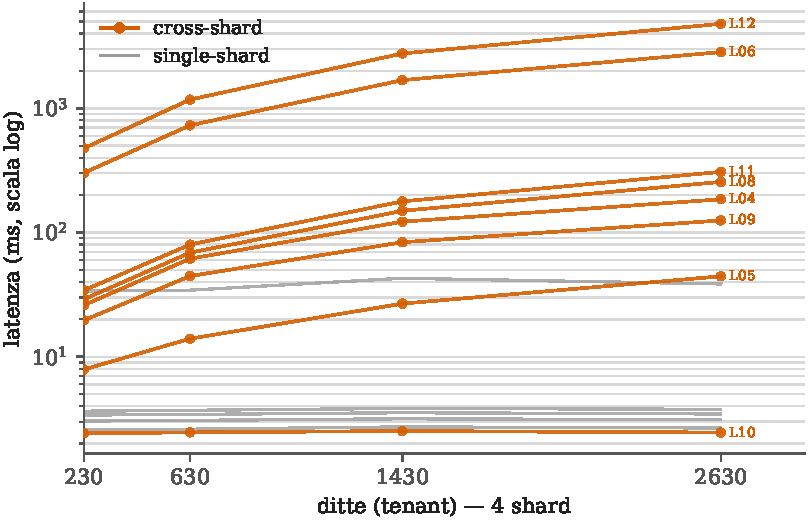
\includegraphics[width=0.82\textwidth]{fig-scaling-dati-mongo}
  \caption{MongoDB, scaling per dati (tutte le 13 letture, 4 shard fissi, scala log): L06 e L12 crescono a
    dismisura col volume, le single-shard restano piatte.}
  \label{fig:mongo-dati}
\end{figure}

\begin{lstlisting}[style=sobrio, language=bash, caption={Esecuzione dello scaling per dati (MongoDB): 4 shard fissi, lotti crescenti di tenant, misura a caldo.}]
export MONGO_PASSWORD=...
bash scala-dati-mongo.sh 64 200 400 800     # +200/+400/+800 tenant -> 230, 630, 1430 ditte
\end{lstlisting}

\subsection{Scritture (MongoDB)}
\label{sec:mongo-scritture}
Le scritture (4 shard, N${=}300$, tenant fisso) confermano la co-locazione e, su U03, producono il contrasto
pro-relazionale più marcato dell'intero lavoro (\Cref{tab:mongo-scritture}). Le scritture \emph{intra-tenant}
(I01, I03, U01, U02, U04) colpiscono \textbf{un solo shard} (quello del tenant): il carico è tutto su
\texttt{10.0.1.4} (CPU ${\sim}5\,\%$), gli altri tre inattivi, esattamente come in Citus. \textbf{U03}
invece, che aggiorna una categoria \emph{denormalizzata} in tutti i cedolini, è un \texttt{updateMany} che
tocca \textbf{tutti e 4 gli shard al 91--99\,\% di CPU}: 356\,ms per operazione e appena 2.8\,op/s. In Citus
la stessa modifica è \textbf{una riga} su una reference table (21\,ms, 47\,op/s): un fattore ${\sim}17\times$
a favore del relazionale.

\begin{table}[htbp]
  \centering
  \caption{MongoDB, scritture a 4 shard (N${=}300$): la co-locazione (una scrittura, uno shard) e il mass-update U03.}
  \label{tab:mongo-scritture}
  \begin{tabular}{llrrl}
    \toprule
    \textbf{Op.} & \textbf{Descrizione} & \textbf{lat (ms/op)} & \textbf{tps} & \textbf{dove scrive} \\
    \midrule
    U02 & licenziamento                & 3.6   & 279 & solo 1 shard \\
    U01 & coordinate bancarie          & 3.6   & 279 & solo 1 shard \\
    U04 & update concorrente           & 3.6   & 277 & solo 1 shard \\
    I01 & inserimento timbratura       & 8.6   & 116 & solo 1 shard \\
    I03 & elaborazione cedolino        & 11.1  & 90  & solo 1 shard \\
    U03 & modifica dato di riferimento & 355.9 & 2.8 & \textbf{tutti i 4 shard (91--99\,\% CPU)} \\
    \bottomrule
  \end{tabular}
\end{table}

\begin{figure}[htbp]
  \centering
  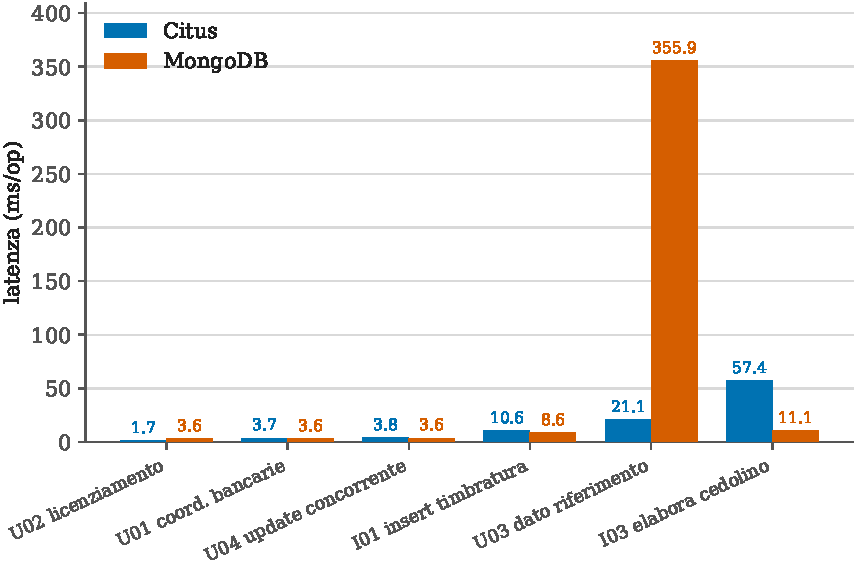
\includegraphics[width=0.85\textwidth]{fig-scritture}
  \caption{Scritture a confronto (4 nodi/shard, N${=}300$): latenza per operazione, Citus vs MongoDB.}
  \label{fig:scritture}
\end{figure}

\begin{lstlisting}[style=sobrio, language=bash, caption={Esecuzione delle scritture (MongoDB): N${=}300$ ripetizioni per query, tenant fisso.}]
bash esegui-scritture-mongo.sh 300 queries/document/scritture/*.js
\end{lstlisting}

\subsection{Comportamento in presenza di guasti (MongoDB)}
\label{sec:mongo-guasti}
Con lo stesso protocollo del test di guasto Citus, si esegue L04 in loop mentre lo shard che ospita i dati
del tenant (\texttt{10.0.1.4}) viene spento e riacceso (10 run). Il comportamento è \textbf{CP}: mentre lo
shard è giù la query fallisce e le righe crollano da 59\,299 a \textbf{0} (nessun risultato parziale), per
tornare al valore pieno al rientro; il recupero è automatico (${\sim}0.25$\,s dopo il riavvio) e
l'indisponibilità dura esattamente il tempo di down (${\sim}15$\,s) (\Cref{tab:mongo-guasti}).

\begin{table}[htbp]
  \centering
  \caption{MongoDB, guasto di uno shard sotto carico di lettura (10 run).}
  \label{tab:mongo-guasti}
  \begin{tabular}{lrrll}
    \toprule
    \textbf{Shard spento} & \textbf{run} & \textbf{error-rate} & \textbf{finestra / recupero} & \textbf{righe (su$\to$giù$\to$su)} \\
    \midrule
    10.0.1.4 (con i dati) & 10 & 7.0\,\% & 10.1$\to$25.2\,s / ${\sim}0.25$\,s & 59\,299 $\to$ \textbf{0} $\to$ 59\,299 \\
    \bottomrule
  \end{tabular}
\end{table}

\begin{figure}[htbp]
  \centering
  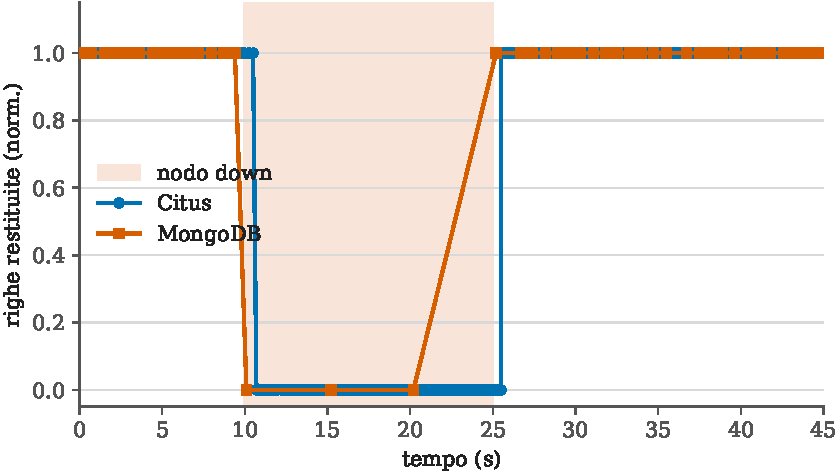
\includegraphics[width=0.8\textwidth]{fig-guasti}
  \caption{Guasto di un nodo sotto carico L04, Citus e MongoDB: righe restituite (normalizzate) nel tempo. In
    entrambi crollano a 0 durante il down (banda) e recuperano al rientro (comportamento CP).}
  \label{fig:guasti}
\end{figure}

Un dettaglio metodologicamente importante: l'error-rate è solo ${\sim}7\,\%$, contro il ${\sim}51\,\%$ di
Citus, \emph{pur avendo la stessa indisponibilità reale} (15\,s). La ragione è il \textbf{diverso
comportamento del client}: il \texttt{mongos} \textbf{si blocca in attesa} dello shard irraggiungibile fino
al timeout (5\,s per operazione), quindi nella finestra di down passano poche operazioni-errore ``lunghe'';
Citus invece \textbf{rifiuta la connessione all'istante} (fail-fast) e ne accumula molte di più. L'error-rate
grezzo non è dunque direttamente comparabile: va letto insieme al \emph{modo} di fallire, cioè \textbf{timeout
bloccanti} in Mongo contro \textbf{errori rapidi} in Citus.

\begin{lstlisting}[style=sobrio, language=bash, caption={Esecuzione del test di guasto (MongoDB): L04 in loop, arresto/riavvio dello shard con i dati.}]
bash test-guasto-mongo.sh queries/document/letture/L04_gender_gap_mediano.js 10.0.1.4 10 15 45
\end{lstlisting}

\section{Confronto tra i due sistemi}
\label{sec:confronto}

Il confronto si articola su più assi (\Cref{tab:confronto,tab:confronto-completo}):
\begin{itemize}
  \item \textbf{Analitica}: dipende dal tipo di query. Dove l'aggregato è servito dall'embedding (percentili
        L04, spesa per categoria L11) MongoDB è più veloce, perché evita le join (a 1 nodo/shard L04 7.2 vs
        71.9\,ms, L11 12.4 vs 75.6\,ms). Ma sulle query che \textbf{attraversano più entità} (assenteismo L06,
        ferie residue L12, riepilogo assenze L13, che toccano assenze e ratei) vince Citus, e di molto: a pari
        scala (${\sim}230$--$240$ ditte, 4 nodi) L06 51 vs 302\,ms, L12 28 vs 476\,ms, L13 3.6 vs 34\,ms.
        MongoDB paga lo scan degli array annidati sull'intera collezione, Citus sfrutta i join indicizzati
        sulle tabelle normalizzate.
  \item \textbf{Scaling}: Citus distribuisce e scala \emph{sempre} (rebalance esplicito, ${\sim}4\times$ con
        4 nodi); MongoDB invece dipende dalla scala: a dati piccoli il balancer non distribuisce (nessuno
        scaling), a volume grande sì (tutti gli shard attivi, cfr.\ \Cref{sec:mongo-dati}).
  \item \textbf{Scritture}: entrambi co-locano la scrittura di un tenant su un solo nodo/shard, ma sul dato
        di riferimento (U03) il relazionale è nettamente più efficiente (1 riga, 21\,ms vs mass-update,
        356\,ms).
  \item \textbf{Guasti}: entrambi CP con la stessa indisponibilità reale, ma \emph{modo} di fallire opposto
        (fail-fast vs timeout bloccante).
  \item \textbf{Query mirate} (cedolino singolo): comparabili (${\sim}$1--2\,ms) su entrambi.
\end{itemize}

\begin{table}[htbp]
  \centering
  \caption{Confronto in latenza (ms) a pari numero di nodi (1) e capacità di scalare.}
  \label{tab:confronto}
  \begin{tabular}{lrrl}
    \toprule
    \textbf{Query} & \textbf{Citus} & \textbf{MongoDB} & \textbf{Scaling coi nodi} \\
    \midrule
    L04 gender gap    & 71.9 & \textbf{7.2}  & Citus ${\sim}4\times$; Mongo no (scala piccola) \\
    L11 spesa/categoria & 75.6 & \textbf{12.4} & Citus ${\sim}4\times$; Mongo no (scala piccola) \\
    L01 cedolino singolo & \textbf{1.5} & 2.3 & entrambi piatti (mirata) \\
    \bottomrule
  \end{tabular}
\end{table}

\begin{figure}[htbp]
  \centering
  \begin{minipage}[t]{0.49\textwidth}
    \centering
    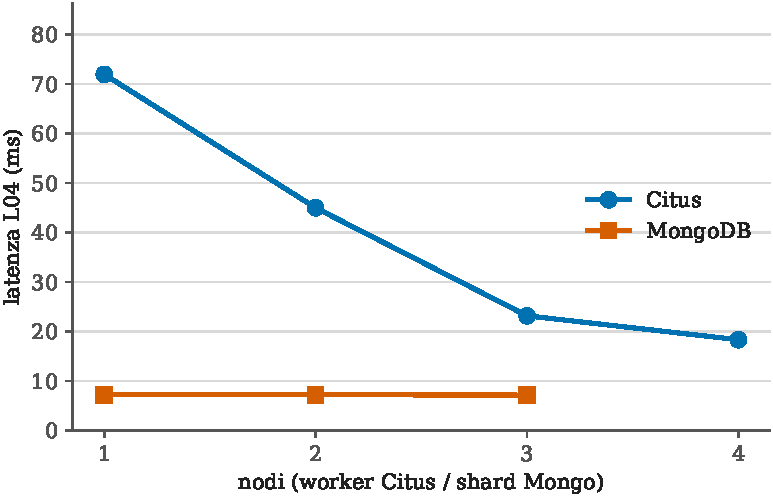
\includegraphics[width=\linewidth]{fig-scaling-nodi-confronto}
    \subcaption{Scaling per nodi su L04: Citus scala, Mongo piatto (scala piccola).}
    \label{fig:scaling-confronto}
  \end{minipage}\hfill
  \begin{minipage}[t]{0.49\textwidth}
    \centering
    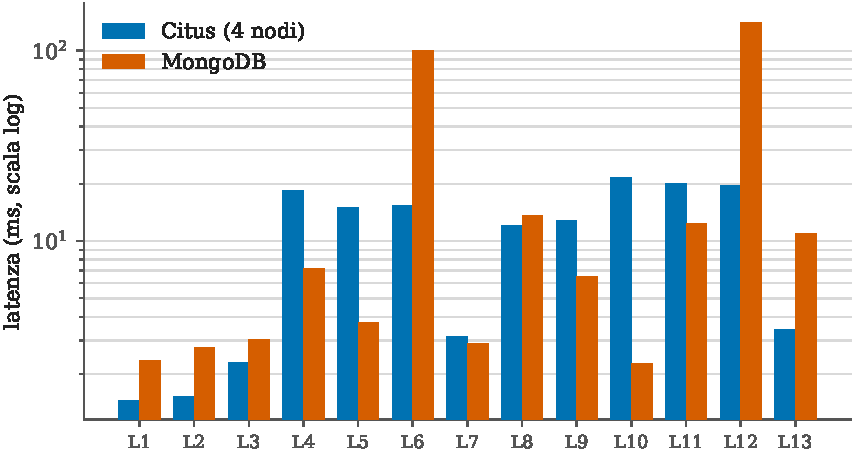
\includegraphics[width=\linewidth]{fig-letture-assolute}
    \subcaption{Latenza assoluta delle 13 letture a scala base (log).}
    \label{fig:letture-assolute}
  \end{minipage}
  \caption{Confronto Citus vs MongoDB: capacità di scalare coi nodi (a) e velocità assoluta in lettura (b).}
  \label{fig:confronto}
\end{figure}

\begin{table}[htbp]
  \centering
  \caption{Confronto complessivo Citus vs MongoDB sui diversi assi misurati.}
  \label{tab:confronto-completo}
  \begin{tabularx}{\textwidth}{@{}lXX@{}}
    \toprule
    \textbf{Aspetto} & \textbf{PostgreSQL + Citus} & \textbf{MongoDB} \\
    \midrule
    Distribuzione dei dati            & esplicita (\texttt{rebalance}, deterministica) & automatica (balancer, soggetta a soglia) \\
    Scaling per nodi (dati piccoli)   & ${\sim}4\times$ con 4 nodi (cross-shard)       & nessuno (balancer sotto soglia) \\
    Scaling per dati (volume grande)  & cross-shard super-lineari                     & idem, e il balancer distribuisce \\
    Analitica sull'aggregato (L04, L11) & più lenta (join)                           & più veloce (embedding) \\
    Query multi-entità (L06, L12, L13)  & \textbf{più veloce} (join indicizzati)     & molto più lenta (array annidati) \\
    Scrittura intra-tenant            & 1 nodo (co-locazione)                         & 1 shard (co-locazione) \\
    Dato di riferimento (U03)         & \textbf{1 riga: 21\,ms, 47\,op/s}             & mass-update: 356\,ms, 2.8\,op/s \\
    Guasto (modo di fallire)          & fail-fast (err ${\sim}51\,\%$)                & timeout bloccante (err ${\sim}7\,\%$) \\
    Guasto (indisponibilità reale)    & ${\sim}15$\,s, recupero ${\sim}0.5$\,s        & ${\sim}15$\,s, recupero ${\sim}0.25$\,s \\
    \bottomrule
  \end{tabularx}
\end{table}

Il confronto diretto sulle \textbf{scritture} (\Cref{tab:confronto-scritture}) dà esiti opposti a seconda
dell'operazione: sull'inserimento del cedolino (I03) è molto più rapido MongoDB (11 vs 57\,ms), perché scrive
un solo documento invece di una transazione su sette tabelle; sull'aggiornamento del dato di riferimento (U03)
è molto più rapido Citus (21 vs 356\,ms), perché tocca una riga su una reference table invece di aggiornare in massa tutti gli
shard. Le scritture semplici (U01/U02/U04) sono equivalenti. Sull'\textbf{analitica}
(\Cref{tab:confronto}) MongoDB è più veloce in assoluto grazie all'embedding.

\begin{table}[htbp]
  \centering
  \caption{Scritture a confronto (4 nodi/shard, N${=}300$): latenza e throughput per operazione.}
  \label{tab:confronto-scritture}
  \begin{tabular}{llrrrr}
    \toprule
    & & \multicolumn{2}{c}{\textbf{Citus}} & \multicolumn{2}{c}{\textbf{MongoDB}} \\
    \cmidrule(lr){3-4}\cmidrule(lr){5-6}
    \textbf{Op.} & \textbf{Descrizione} & \textbf{ms/op} & \textbf{op/s} & \textbf{ms/op} & \textbf{op/s} \\
    \midrule
    U02 & licenziamento          & 1.7  & 605 & 3.6   & 279 \\
    U01 & coordinate bancarie    & 3.7  & 273 & 3.6   & 279 \\
    U04 & update concorrente     & 3.8  & 266 & 3.6   & 277 \\
    I01 & inserimento timbratura & 10.6 & 94  & 8.6   & 116 \\
    I03 & elaborazione cedolino  & 57.4 & 17  & \textbf{11.1}  & \textbf{90} \\
    U03 & dato di riferimento    & \textbf{21.1} & \textbf{47} & 355.9 & 2.8 \\
    \bottomrule
  \end{tabular}
\end{table}

Il contrasto tra i modelli si vede meglio sulle coppie deliberate. Il \textbf{cedolino completo} è
pro-documentale: una \texttt{findOne} su un documento (\Cref{lst:l10-mongo}) contro l'assemblaggio da sette
tabelle in Citus. Il \textbf{dato di riferimento} è pro-relazionale: una riga su una reference table
(\Cref{lst:u03-citus}) contro un \texttt{updateMany} di centinaia di documenti denormalizzati in Mongo.

\begin{lstlisting}[style=sobrio, language=Java, caption={Cedolino completo in MongoDB: un solo documento (pro-documentale).}, label={lst:l10-mongo}]
db.cedolini.findOne({ tenant_id: 1, dipendente_id: 7, anno: 2026, mese: 6 });
\end{lstlisting}

\begin{lstlisting}[style=sobrio, language=SQL, caption={Modifica di un dato di riferimento in Citus: una riga (pro-relazionale).}, label={lst:u03-citus}]
UPDATE tipo_voce SET categoria = 'WELFARE' WHERE codice = '0401';   -- 1 riga (in Mongo: updateMany su N documenti)
\end{lstlisting}


% 6. Conclusioni: quando conviene ciascun sistema, limiti
\chapter{Conclusioni}
\label{ch:conclusioni}

Il lavoro ha confrontato, sullo stesso dominio HR/retributivo e sulla stessa infrastruttura, un relazionale
distribuito (PostgreSQL+Citus) e un documentale (MongoDB), entrambi CP ma con modelli di dati opposti. Ne
emerge che la domanda ``quale sistema è migliore'' non ha risposta assoluta: dipende dall'operazione e dalla
scala, coerentemente con l'idea che non esista una taglia unica~\cite{stonebraker2005onesize}.

\section{Sintesi dei risultati}
\label{sec:sintesi}

\begin{itemize}
  \item \textbf{Scalabilità per nodi (Citus)}: le analitiche cross-shard scalano quasi linearmente
        (${\sim}3.8\text{--}4.6\times$ con 4 nodi); le query mirate a un tenant restano piatte perché
        colpiscono un solo shard, ma sono già nell'ordine del millisecondo. Il miglioramento è più marcato
        proprio per le query che aggregano e uniscono (join) dati di più tenant, come mostrano
        \Cref{tab:scaling-nodi,tab:scaling-nodi-full}: la L05, ad esempio, arriva a $4.4\times$ passando da 1
        a 4 nodi.
  \item \textbf{Scalabilità per dati (Citus)}: a nodi fissi le cross-shard degradano super-linearmente col
        volume, mentre le single-shard restano insensibili grazie all'indicizzazione e alla co-locazione per
        tenant.
  \item \textbf{Scritture (Citus)}: la co-locazione fa sì che la scrittura di un tenant colpisca un solo nodo;
        solo la modifica di un dato di riferimento tocca tutti i nodi. La transazione multi-tabella è
        l'operazione più costosa.
  \item \textbf{Guasti}: comportamento \textbf{CP} confermato; con un nodo giù la query cross-shard
        fallisce per l'intera finestra (nessun risultato parziale), con recupero automatico e rapido al
        rientro. La consistenza è scelta al posto della disponibilità.
  \item \textbf{MongoDB}: più veloce sulle analitiche che l'embedding serve direttamente (percentili, spesa
        per categoria), ma \textbf{nettamente più lento} sulle query che attraversano più entità (assenteismo,
        ferie residue, che toccano assenze e ratei): lì Citus, con i join indicizzati, è risultato più rapido
        di 6--17 volte a pari scala. Inoltre il balancer, volutamente conservativo, \textbf{non distribuisce a
        scala piccola}, quindi a quella scala aggiungere shard non porta beneficio; la distribuzione riparte
        solo a volume grande, in contrasto con il rebalance esplicito e deterministico di Citus.
  \item \textbf{Modellazione}: il cedolino completo premia il documentale (un documento vs sette tabelle),
        mentre il dato di riferimento e le aggregazioni multi-entità premiano il relazionale (una riga vs
        aggiornamento di massa; join indicizzati vs scan di array annidati).
\end{itemize}

\section{Quando conviene ciascun sistema}
\label{sec:quando}

Sulla base delle misure: \textbf{Citus} è preferibile quando servono analitiche cross-tenant che devono
\emph{scalare} orizzontalmente in modo prevedibile e, soprattutto, per le \textbf{query complesse che
attraversano più entità} (aggregazioni e join profondi su assenze, ratei, contratti): proprio lì, dove
MongoDB deve scorrere gli array annidati sull'intera collezione, Citus è risultato molte volte più veloce a
pari scala. Si aggiungono l'integrità referenziale forte, le transazioni distribuite e il controllo esplicito
della distribuzione tipico di un DBA. \textbf{MongoDB} è preferibile quando il
carico è dominato da operazioni sull'\emph{aggregato} (lettura/scrittura del documento completo), quando conta
la bassa latenza sulle singole richieste e la flessibilità di schema, accettando in cambio un controllo meno
fine sulla distribuzione e la denormalizzazione dei dati condivisi.

\section{Limiti e sviluppi futuri}
\label{sec:limiti}

I risultati vanno letti alla luce di alcuni limiti dichiarati. La scala è dell'ordine dei GB (vincolo del
disco delle VM), non delle centinaia di GB. Il working set è sempre rimasto in RAM (cache di Postgres e di
WiredTiger): le letture da disco sono state nulle, quindi il regime I/O-bound non è stato raggiunto. Gli
esperimenti si sono fermati quando la tendenza era già chiara e i dati risultavano distribuiti su tutti i
nodi, senza spingersi fino a saturare il disco. Entrambi i sistemi sono inoltre a copia singola (nessuna
replica), scelta voluta per un test di guasto CP corretto ma che esclude l'alta disponibilità.

Come sviluppi: spingere i volumi fino alla saturazione effettiva del disco per osservare il regime I/O-bound;
introdurre la replica per confrontare disponibilità e comportamento in failover; e misurare esplicitamente
uno scenario di evoluzione di schema (turni/ferie) su entrambi i sistemi, oggi trattato solo a livello teorico.


\clearpage
\printbibliography[heading=bibintoc]

\end{document}
